\chapter{Renormalization and effective field theory}
\section{Renormalization and effective field theory}
\label{sec:renormalization}
Approaches to \emph{Renormalization}:
\begin{enumerate}
	\item[$1)$] Renormalization of quantum potential
	\item[$2)$] On-shell renormalization of scattering amplitudes (classification by degree of divergence)
	\item[$3)$] Callan-Symanzik flow equation (perturbative flow of correlators, computation of $\beta$-functions)
	\item[$4)$] Wilsonian effective field theory (flow of UV cut-off regularized theories)
	\item[$5)$]functional RG (flow of IR mass regularized quantum vertices)
\end{enumerate}
Methods $1-3$ are perturbative and we are free to pick our \emph{regularization} scheme, e.g.
\begin{enumerate}
\item[$\bullet$] Cut-off regularization ($\int^\infty \rightarrow \int^\Lambda$)
\item[$\bullet$] Dimensional regularization ($\md^d p \rightarrow \md^{d-\epsilon} p$)
\item[$\bullet$] Pauli-Villars regularization ($k^2\rightarrow k^2-\mu^2$)
\end{enumerate}
while methods $4$ and $5$ come with their own regularization schemes. The regularization schemes for perturbative renormalization are detailed in \ref{subsec:renormalizationRegSchemes}. The fourth and fifth method are discussed in their own chapters.\\
\\
Callan-Symanzik's method derives a flow equation from the demand for consistency of an arbitrary renormalization scheme.\\
Wilson's method introduces a UV cut-off and applies the spin block renormalization idea as a transformation of Lagrangians where we are free to interpret theories with a finite cut-off as effective theories.\\
The FRG finally introduces regularization at the non-perturbative level of the quantum action and is able to derive all correlation functions from flow equations.\\
\\
There have been two fundamental insights in the development of
the renormalization group. One, due to Gell-Mann and Low, is
that logarithms of energy that violate naive scaling and invalidate perturbation theory arise because of the way that renormalized coupling constants are defined, and that these logarithms
can be avoided by renormalizing at a sliding energy scale. The
second fundamental insight, due to Wilson, is that it’s very important in dealing with phenomena at a certain energy scale to
integrate out the physics at much higher energy scales. These insights are conceptually not that different, because when you adopt the
Gell-Mann–Low approach and define a renormalized coupling
at a sliding scale and use renormalization theory to eliminate
the infinities rather than an explicit cutoff, you are in effect integrating out the higher energy degrees of freedom — the integrals
converge because after renormalization the integrand begins to
fall off rapidly at the energy scale at which the coupling constant
is defined. (This is true whether or not the theory is renormalizable in the power-counting sense.) So in other words instead of
a sharp cut-off a la Wilson, you have a soft cut-off, but it’s a cut-off
nonetheless and it serves the same purpose of integrating out the
short distance degrees of freedom.
\\
\\
An overarching result of all methods is that renormalizability is an emergent quality of quantum field theories that is a result of testing it experimentally in the IR, where non-renormalizable interactions are irrelevant. The tricky part is the distinction between \emph{perturbative renormalizability} (done by power counting degree of divergences and computation of anomalous dimensions in loop expansions) and \emph{non- perturbative} (read ’true’) \emph{renormalizability} (done by proving the existence of asymptotically save fixed points). For example QED and $\phi^4$-theory, even though perturbatively renormalizable by degree of divergence, are non- perturbatively non- renormalizable manifest by appearance of Landau poles in the UV. A well established result at this point is that QCD and YM theory are truly renormalizable by virtue of UV save fixed points and confinement preventing IR divergencies. A less established result of the FRG is that gravity also has a UV save fixed point and is thereby non-perturbatively renormalizable despite being perturbatively non-renormalizable.


\subsection{Mass dimension}
\begin{mybox}{Definition and calculation}
	Since we work in $\hbar=c=1$ the only dimension left is the mass dimension, which we define by
	\begin{equation}
		[c(\text{mass unit})^n] :=n \text{ for } c\in \mathbb{C}
	\end{equation}
	which is Lorentz-invariant since mass $m^2=p^2$ is a Lorentz-scalar. This also immediately gives us
	\begin{equation}
		[p]=1.
	\end{equation}
	Because the mass dimension extracts the exponent of the mass unit
	\begin{equation}
	[AB] = [A] + [B]
		\end{equation}
which is a special case also gives us
\begin{equation}
	[A^n] = n [A].
\end{equation}
$p^\mu x_\mu$ is a number, i.e. $[px]=0$ so
\begin{equation}
	[x]=[\md x] = -1,\quad [\partial] =1.
\end{equation}
We want the action to be a fundamental object that does not need to refer to a scale and can be taken as the argument of functions we demand
\begin{equation}
	[S]\stackrel{!}{=}0,\quad [\mL]=d.
\end{equation}
Since addition is defined between objects of the same mass dimension
\begin{equation}
	[A+B] = [A] = [B]
\end{equation}
so we can extract mass dimensions of objects in an action summand by summand.
\end{mybox}
\begin{mybox}{Explicit examples}
The kinetic term of any field theory only contains differentials and fields. We know the mass dimension dimension of the differentials and the action so we can extract the mass dimension of any field from the kinetic term. For the scalar $\phi$, Dirac $\psi$ and Yang-Mills field $A$ we obtain
\begin{equation}
	[\phi] = [A] = \frac{d-2}{2},\quad [\psi] = \frac{d-1}{2}
\end{equation}
ie. in $d=4$
\begin{equation}
[\phi] = [A] =1, \quad [\psi]=\frac{3}{2}.
\end{equation}
Knowing the mass dimensions of the field, we can extract the mass dimension of any coupling from the potential terms. For $\phi^n$ theory in $d$ dimensions we obtain
\begin{equation}
	[\lambda_n] = d-n[\phi] = (1 -\frac{n}{2}) d+n,
\end{equation}
for Yukawa theory and Yang-Mills theory (including QED) 
\begin{equation}
	[g] = 2 - \frac{d}{2}.
\end{equation}
\end{mybox}
Other useful mass dimensions are:
\begin{align}
	[\frac{1}{\xi}] &=0\quad  \text{(Gauge fixing parameter of Yang-Mills)}\\
	[\lambda_n] &= 4-n \quad (\phi^n \text{ in } d=4)\\
	[\lambda_4] &= 4-d \quad (\phi^4 \text{ in arbitrary } d)\\
	[\lambda_3] &= 3-\frac{d}{2} \quad (\phi^3 \text{ in arbitrary } d).
\end{align}
For mass dimensions of GR see \todo{reference here}.\\
\\
Derivation of mass dimensions:
\begin{enumerate}
	\item Scalar field mass dimension:
	\begin{align*}
		0 &\stackrel{!}{=} \left[\int \md^d x \partial_\mu \phi \partial^\mu \phi\right] = [\md^d x \partial_\mu \partial^\mu \phi]\\
		&= d [x] + 2 [\partial] + 2 [\phi] \\
		&= -d +2 +2 [\phi] \quad \Leftrightarrow\; [\phi] = \frac{d-2}{2}.
	\end{align*}
\item Dirac  field mass dimension:
\begin{align*}
	0&\stackrel{!}{=} [\md^d x \bar{\psi} i \gamma^\mu \partial_\mu \psi] \equiv [\md^d x (\psi^\dagger)^A (\gamma_0)^{AB} i (\gamma^\mu)^{BC} \partial_\mu \psi^C]\\
	&= d[x] + [(\psi^\dagger)^A]+ [(\gamma_0)^{AB} i (\gamma^\mu)^{BC} ] + [\partial] + [\psi^C] \\
	&= d [x] = 2 [\psi] + [\partial] \\
	&= -d +2 [\psi] +1 \quad \Leftrightarrow \; [\psi] = \frac{d-1}{2}.
\end{align*}
\item Yang-Mills field mass dimension
\begin{align*}
	0&\stackrel{!}{=} [\md^d x \tr F^{\mu \nu} F\munu] = d[x] + [F^{\mu \nu}_a F^a\munu] \\
	&= d[x] + [\partial^\mu A^\nu_a \partial_\mu A^a_\nu] \\
	&= d [x] + 2[\partial] + 2 [A] \\
	&=-d +2 +2 [A] \quad \Leftrightarrow \; [A] = \frac{d-2}{2}.
\end{align*}
\end{enumerate}


\subsection{Classification of operators}
Lagrangians are fixed by the requirement of gauge-invariance and renormalizability. One ca classify operators which you can add to the Lagrangian in $d=4$ as
\begin{enumerate}
	\item $[\mO] >4$ are called \emph{irrelevant} as they are non-renormalizable.
	\item $[\mO] =0$ are called \emph{marginal} as they are not relevant operators in terms of physics.
	\item $[\mO]<4$ are called \emph{relevant} as these terms in the Lagrangian are (super-) renormalizable.
\end{enumerate}
\subsection{Topological classification of diagrams (graph theory)}
\begin{mybox}{}
	We define
	\begin{align}
		E&:= \#(\text{external lines})\\
		I&:= \#(text{internal lines})\\
		L&:=\#(\text{loops}) \\
		V&:=\#(\text{vertices})
	\end{align}
such that we can define the following identities:
\begin{enumerate}
\item Identities for $\phi^n$-theory
\begin{align}
L&=I-V+1 \\ 
n \cdot V &= 2I+E 
\end{align}
\item Identities for QED
\begin{align}
	L&=I_e+I_\gamma -V+1 \\
	2V&= E_e + 2I_e \\
	V&= E_\gamma + 2 I_\gamma.
\end{align}
\end{enumerate}
\end{mybox}
Note that an expansion in $L$ for fixed $E$ is equivalent to an expansion in $V$ and thereby to an expansion in $\lambda$
\begin{equation}
	(n-2)V=2L+E-2.
\end{equation}
An expansion in $\lambda$ gives
\begin{equation}
	I-V = L-1 \quad \text{powers of } \hbar.
\end{equation}







\subsection{Superficial degree of divergence and renormalizability}
\begin{mybox}{Renormalizability}
	A general QFT is called renormalizable if only a finite number of resummed amputated $1PI$ diagrams is UV divergent.
\end{mybox}
Suppose the renormalizable QFT contains $m$ different fields and suppose that the UV divergent $1PI$ diagrams give rise to $n$ divergent constants order by order in perturbation theory. Then $(n-m)$ of these constants can be absorbed in the definition of $(n-m)$ unphysical parameters, the so-called \emph{bare couplings.}\\
This procedure requires specifying the outcome of $(n-m)$ physical observables as external input, i.e. experiment $\Rightarrow$ bare couplings. The remaining $m$ constants can be absorbed in the definition of the kinetic terms of the $m$ fields without reducing the predictability of the theory further. Thus in a renormalizable theory only a finite number $(n-m)$ of physical observables must be specified order by order in perturbation theory, and predictive power is retained for all remaining observables, which can e computed and are finite as we remove the cutoff.\\
However, the price to pay for the appearance of the UV divergences in the first place is that the $(n-m)$ observables cannot be computed by the theory even in principle! For instance, QED cannot make any predictions whatsoever for the absolute value of the electron mass or the charge at $q^2=0$. However, once we take $e(q^2=0)$ from experiment, QED does predict the logarithmic running of the effective charge as a function of $q^2$. As a result the renormalized QFT necessarily contains free parameters that must be fitted to experiment. Another example for such an observable for which no prediction can be made in QFT with divergent partition function is the vacuum energy (cosmological constant). A non-UV finite, but renormalizable QFT is an \emph{effective theory}: The UV divergences hint at a breakdown of the theory at high energies where it does not describe the microscopic degrees of freedom correctly. Renormalization hides our ignorance about the true physics at high energies in the $(n-m)$ observables and we can fit the theory to experiment as one typically does with a phenomenological model.
\\
\\
\begin{mybox}{Superficial degree of divergence}
The  \emph{superficial degree of divergence} $D$ of $\mathcal{D}$ is defined as the difference in powers of momentum between numerator and denominator, i.e.
\begin{align}
	D&= (\text{power of momenta in numerator}) \\
	&- (\text{power of momenta in denominator})\nonumber \\
			\phi^n \Rightarrow \quad D &= \md L - 2 I.
\end{align}
E.g. for a scalar theory in $d$ dimensions with (bare) Lagrangian $\mL_0 = \half (\partial \phi)^2 - \frac{m^2_0}{2} \phi^2 - \frac{\lambda_0}{n!} \phi^n$, the naive UV structure of a diagram $\mathcal{D}$ with $L$ loops $\propto \int_{\mR^d} \md^d k$ and $I$ propagators $\propto (k^2-m^2)^{-1}$ is 
\begin{equation}
\mathcal{D} \stackrel{k\rightarrow\infty}{\rightarrow} \underbrace{\int_{\mR^d} \md^d k_1 \dots \int_{\mR^d} \md^d k_L  }_{\times L} \underbrace{\frac{1}{k^2_1 \dots k^2_I} }_{\times I}.
\end{equation}
\end{mybox}
\begin{enumerate}
	\item Regularizing the divergence with a momentum cutoff $\Lambda$, i.e. $\int_{-\infty}^{\infty} \md k \rightarrow \lim_{\Lambda \rightarrow\infty} \int_{-\Lambda }^{\Lambda} \md k$, diagrams fall into three categories of UV behaviour if we are talking about the naive scaling behaviour of amplitudes $\mM$ under cut-off regularization
	\begin{enumerate}
		\item $D>0 \quad \Rightarrow \, \mathcal{M}\propto \Lambda^D$ \emph{superficially  divergent}
		\item $D<0 \quad \Rightarrow \, \mathcal{M}\propto \Lambda^{-|D|}$ \emph{superficially finite}
		\item $D=0 \quad \Rightarrow \, \mathcal{M}\propto \ln(\Lambda)$ \emph{superficially log-divergent}
	\end{enumerate}

According to this reasoning, as $\Lambda \rightarrow\infty$ only diagrams with $D\geq0$ are divergent. Therefore $D$ is called superficial degree of divergence: The term superficial indicates that $D$ does not always reflect the actual divergence or finiteness properties of a diagram, due to these 3 possible reasons listed above.
\item The actual UV-behaviour may differ from the superficial one for three reasons:
\begin{enumerate}
	\item For $D\geq 0$, a diagram may still be actually finite if a sufficient amount of symmetry constrains the form of the amplitude or leads to cancellations among infinite terms.
	\item For $D<0$, a diagram may still be divergent if it contains a divergent subdiagram.
	\item Tree-level diagrams have $D=0$, but are finite.
\end{enumerate}
\end{enumerate}



\begin{mybox}{Topological relations}
	Expressing the superficial degree of divergence in terms of number of loops $L$, number of internal lines $I$, number of $n$-field vertices $V_n$
	\begin{equation}
		D = dL - [(\text{propagator})] I - \sum_{n=3}^{\infty} [(n-\text{vertex})] V_n
	\end{equation}
	we have the general graph theory (topology) relations
	\begin{equation}
		E+2I = \sum_{n=3}^{\infty} n V_n,\qquad L = I+1-\sum_{n=3}^{\infty}V_n,
	\end{equation}
	 identities for $\phi^n$-theory in $d$ dimensions ($d$ enters via integral measure, only one kind of vertex present $V_n=V$)
	\begin{align}
		D&= d \cdot L - 2I\\
		D&= d + \left(n\frac{d-2}{2}-d\right) \cdot V-\frac{d-2}{2} E = d - [\lambda^{(n)}] \cdot V - [\phi] E,
	\end{align}
and the identity for QED in $d=4$
\begin{equation}
	D=4L-I_e-2I_\gamma.
\end{equation}
QED has a finite number of superficially divergent amplitudes
\begin{equation}
D=4-\frac{3}{2}E_e-E_\gamma
\end{equation}
namely amplitudes with$\frac{3}{2}E_e+E_\gamma \leq 4$ $\Leftrightarrow$ $3 E_e+2 E_\gamma \leq 8$.\\
The superficial degree of divergence is only a rule of thumb when it comes to actual divergences and 
\begin{align}
	&\text{symmetry can prevent superficial divergence }\nonumber \\
	&\Rightarrow \text{divergence}\\
	&\text{divergent subdiagrams can prevent superficial divergence }\nonumber \\
	& \Leftarrow \text{divergence}
\end{align}
\end{mybox}
The superficial degree of divergence in other useful theories are
\begin{align}
	D&= 4+(n-4)V-E \quad (\phi^n \text{ in } d=4) \\
	D&= d+(d-4)V-(\frac{d}{2}-1) E \quad (\phi^4 \text{ in arbitrary } d) \\
	D&= d+(\frac{d}{2} -3)V-(\frac{d}{2}-1)E \quad (\phi^3 \text{ in arbitrary } d).
\end{align}
\begin{enumerate}
	\item $\phi^4$ theory in $d=4$ has a \emph{finite} number of superficially divergent \emph{amplitudes}
	\begin{equation}
	\label{eq:renormalizationSdodphi4}
	D=4-E
	\end{equation}
	namely amplitudes with $E\leq 4$.
	\item $\phi^3$ theory in $d=4$ as a \emph{finite} number of superficially divergent \emph{diagrams}
	\begin{equation}
		D=4-V-E
	\end{equation}
	namely diagrams with $E+V\leq 4$.
	\item $\phi^5$ theory in $d=4$ has an \emph{infinite} number of superficially divergent amplitudes
	\begin{equation}
		D=4+V-E
	\end{equation}
because for fixed $E$ every amplitude gets divergent contributions from diagrams with $V \geq 4-E$.
\item Note that Yukawa theory (with $V(\phi)\equiv 0$) behaves exactly as QED with the photon being replaced by the scalar particle, because the interaction terms of the same form $A^\mu \bar{\psi} \psi \leftrightarrow\phi \bar{\psi} \psi$, such that for Yukawa theory
\begin{equation}
\label{eq:renormalizationSdodYukawa}
	D=4-\frac{3}{2}E_e-E_\phi.
\end{equation}
\item A QED diagram with $E_e(E_{\gamma})$ external fermions (photons) has superficial degree of divergence
\begin{equation} 
\label{eq:renormalizationSdodQED}
D = 4- E_{\gamma} - \frac{3}{2} E_e.
\end{equation}
\item The SDOD for QCD is given by 
\bse 
D(G) = \md \cdot L - I_q-2 I_g -2 I_u + V_u + V_{3 \text{ gluon}},
\ese 
where $q$ indicates quarks, $g$ indicates gluons and $u$ indicates ghosts. With the following topological relations
\begin{align*}
	L &= I_{all} - V_{all} +1, \quad 2 I_u + E_u = 2 V_u \\
	2 I_g + E_g &= V_q + 3 V_{3 g} + 4 V_{4 g} + V_u
\end{align*}
we find in $\md=4$
\be 
\label{eq:renormalizationSdodQCD}
D(G) = 4-E_g - \frac{3}{2} E_q - E_u.
\ee 

\end{enumerate}


\subsection{Perturbative renormalizability and classification of couplings}
\begin{mybox}{Renormalizability}
	The UV properties of a theory are decisively determined by (the sign of) the prefactor of V.
\end{mybox}
Thus, following this reasoning:\\
$\lambda^{(4)}_0$ is scale independent, $\lambda^{(5)}$ is $\propto \frac{1}{E}$ thus IR dominant and $\lambda^{(3)}$ is $\propto E$, thus UV dominant.
\begin{mybox}{Renormalizability}
	\begin{enumerate}
		\item
	A theory is called \emph{power-counting renormalizable} if the number of superficially divergent amplitudes is finite, but superficial divergences appear at every order in perturbation theory.
	\begin{statements}
		$\stackrel{D}{\Leftrightarrow}$ power-counting renormalizable if its coupling has vanishing mass dimension, e.g. $\phi^4$.
	\end{statements}
\item A theory is called \emph{power-counting super-renormalizable} if the number of superficially divergent Feynman diagrams is finite.
\begin{statements}
	$\stackrel{D}{\Leftrightarrow}$ power-counting super-renormalizable if its coupling has positive mass dimension, e.g. $\phi^3$.
\end{statements}
\item A theory is called \emph{power-counting non-renormalizable} if the number of superficially divergent amplitudes is infinite
\begin{statements}
	$\stackrel{D}{\Leftrightarrow}$ power-counting non-renormalizable if its coupling has negative mass dimension, e.g. $\phi^5$.
\end{statements}
\end{enumerate}
\end{mybox}
\begin{mybox}{Power-counting renormalizability of $\phi^n$-theory}
	\begin{align}
	\phi^n \text{ is renormalizable } &\Leftrightarrow [\lambda^{(n)}_0] = 0 \\
	\phi^n \text{ is non-renormalizable } &\Leftrightarrow [\lambda^{(n)}_0] <0 \\
	\phi^n \text{ is super-renormalizable } &\Leftrightarrow [\lambda^{(n)}_0] > 0. 
	\end{align}
\end{mybox}
Altogether:
\begin{enumerate}
	\item $\Leftrightarrow$ If $D\propto + V$, there exists an infinite number of $E$, superficially divergent amplitudes since for every ??, diagrams with high enough $V$ diverge. The theory is thus \emph{non-renormalizable} $\Leftrightarrow [\lambda_0] <0$.
	\item If $D\slashed{\neq} V$ (and $\md \geq 2$), only a finite number of diagrams is divergent but divergences appear at every loop-order. Such theories are called \emph{renormalizable} and arise for $[\lambda]=0$.
	\item If $D \propto -V$, for high-enough loop order, all diagrams become superficially finite, making the theory \emph{super-renormalizable} $\Leftrightarrow [\lambda_0] >0$.
\end{enumerate}
E.g. for $n=d=4$, we have $[\lambda_0 ] =0$ and $D=4-E$ independent of $L$ or $V$. Hence, $\phi^4$-theory in $d=4$ is renormalizable with only three superficially divergent diagrams (\emph{at every loop order}).

\subsection{Renormalization theorem (BPHZ theorem)}
\begin{mybox}{BPHZ in a nutshell}
	If a theory is power-counting renormalizable, i.e. has a finite amount of superficially divergent amplitudes, at each order in perturbation theory only a finite number of divergent diagrams, parametrized by a finite number of divergent constants, appear. One can absorb these
	divergences order by order in the counterterms introduced in the reparametrization of the Lagrangian such that all
	physical amplitudes are finite.\\
	This is because the counterterms create new Feynman diagrams relevant at the next order. These will cancel
	the divergences of the divergent subdiagrams (if present) at the next order.\\	
	All of this leads to a perturbative adjustment of a finite number of counterterms in the renormalised Lagrangian, and thus predictivity is maintained.
\end{mybox}

By the BPHZ theorem, (power counting) renormalizability is sufficient for a theory to maintain predictability. The non-trivial aspect of this theorem concerns the complete cancellation of divergent subdiagrams by counterterms of the previous loop order (example $\phi^4$ theory to $2$nd-loop renormalized). The proof is apparently very involved.\\
\\
There is another theorem by 't Hooft and Veltman, which states that infinities are governed by the same
gauge symmetries as the terms in the Lagrangian. This was originally proven only for theories that are renormalizable in
the old power-counting sense, but this theorem has only recently
been extended to theories of the Yang–Mills or Einstein type
with arbitrary numbers of complicated interactions that are not
renormalizable in the power-counting sense.


\subsection{A more in-depth look at regularization schemes}
\label{subsec:renormalizationRegSchemes}
\begin{mybox}{Regularization}
	Regularization is the practice of isolating divergences. The three common methods in QFT are:
	\begin{enumerate}
		\item 1) \emph{Cutoff regularization}: regularizes divergent momentum integrals via $\int_{-\infty}^{\infty} \md k \rightarrow \lim_{\Lambda \rightarrow\infty} \infty_{-\Lambda}^{\Lambda} \md k$. However, this is for QED inconsistent with the Ward identities and gauge invariance because transformations of the sort $A^{\mu} \rightarrow A^{\mu} + \partial^{\mu} \alpha(x)$ cannot be carried out at the cutoff, making it a useless method in QED.
	\item \emph{Dimensional regularization}: evaluates divergent integrals in $\md =4-\epsilon$ dimensions. The result is expanded in power of $\epsilon$, which isolates the divergence as a pole as $\epsilon \rightarrow 0$.
	\item \emph{Pauli-Villars regularization} takes a divergent diagram and subtracts it from the same diagram, but with a fictitious massive particle in the loop, e.g. a photon of mass $\Lambda$.\\
	This removes the divergence, because for $k\rightarrow\infty$ the mass in the loop becomes irrelevant and both diagrams asymptote to the same value.\\
	But for $\Lambda \rightarrow \infty$, the auxiliary diagram vanishes and we recover the actual process.
	\end{enumerate}
\end{mybox}
\subsubsection{Dimensional regularization}
\label{subsubsec:renormalizationDimReg}
The \emph{dimensional regularization} can be used in the context of the following steps
\begin{enumerate}
	\item The integrand of the loop integral contains a fraction of the form $\frac{1}{AB}$ with e.g. $A=(p-k)^2-\mu^2+i \epsilon$ and $B=k^2-m^2_0+i\epsilon$. Transform momentum dependent integrand via \emph{Feynman parametrization},  which is satisfied for any $A,B \in \mathbb{C}\ \{0\}$ 
	\begin{equation}
		\int_0^1 \md x \frac{1}{[xA+(1-x)B]^2} = \frac{1}{AB}.
	\end{equation}
	\item Shift the integration variable 
	\begin{equation*}
		l:= (k \pm xp) \quad \Rightarrow \quad \md l=\md k.
	\end{equation*}
	\item Impose dimensional regularization by going over to $\md=4-\epsilon$ dimensions.
	\item We now encounter loop-integrals of the typical form $\int \frac{\md^4 l}{(2 \pi)^4} \frac{1}{(l^2-\Delta +i \epsilon)^n}$, which can be easily solved by a \emph{Wick rotation} to Euclidean space.	The $^0$ integral is in fact a complex contour integral along the real axis. The value of this integral is unchanged if we deform the contour without hitting any pole. Therefore we can rotate the contour by $90^°$ counter-clockwise to lie along the imaginary axis:
	\begin{figure}
		\centering
		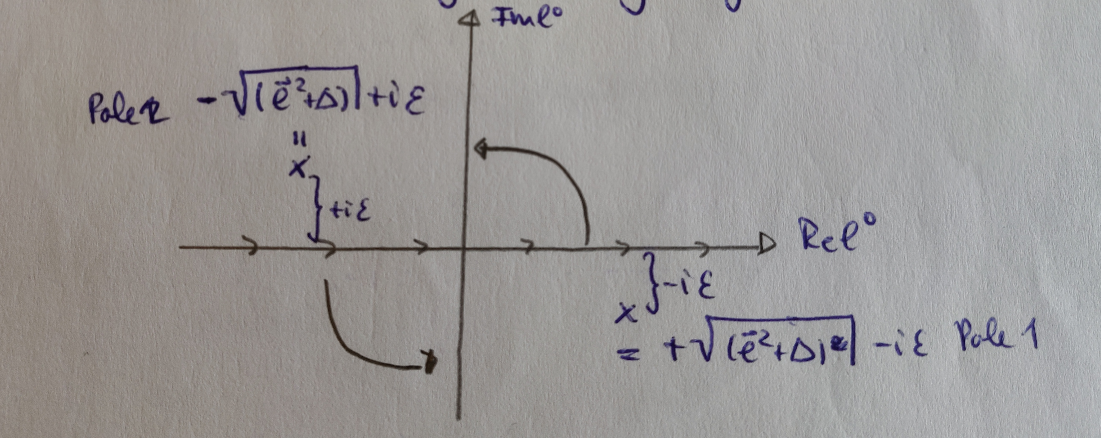
\includegraphics[width=0.7\linewidth]{gfx/Wickrotation}
		\caption{\itshape How to perform integral in the renormalization procedure by a Wick rotation.}
		\label{fig:wickrotation}
	\end{figure}

	Introducing the Euclidean $4$-momentum $l_E = (l^0_E, \vec{l}_E)$ as 
	\begin{equation}
	l^0=i l^0_E, \; \vec{l}=\vec{l}_E \; \Rightarrow \; l^2=-l^2_E\equiv \; -i \sum_j (l^j_E)^2, \; \frac{i}{l^2-m^2}=\frac{1}{l^2_E+m^2}.
	\end{equation}
	We can write the integral as
	\begin{equation}
	\int \frac{\md^4 l}{(2 \pi)^4} \, \frac{1}{[l^2-\Delta+i\epsilon]^m} = (-1)^m i \int \frac{\md^4 l}{(2 \pi)^4} \, \frac{1}{[l^2_E+\Delta - i \epsilon]^m}.
	\end{equation}
	Since we won't need the $i\epsilon$ any longer we can omit it at this stage. We can now perform the integral as a spherical integral in $\mR^{\md}$.
	
	\item  Carry out the loop-integral in $\md$-dimensional spherical coordinates
	\begin{equation}
		\int \frac{\md^{\md}l_E}{(2\pi)^{\md}} = \int \md \Omega_{\md} \int_0^\infty \frac{\md l_E}{(2 \pi)^{\md}} l^{\md-1}_E
	\end{equation}
	where the area of the $\md$-dimensional unit sphere is given by
	\begin{equation}
		\int \md \Omega_{\md} = \frac{2 \pi^{\frac{\md}{2}}}{\Gamma(\frac{\md}{2})}
	\end{equation}
	\item Substitute 
	\begin{equation*}
		x= \frac{m^2}{l^2_E+m^2} \quad \Rightarrow \quad \md x = - \frac{2 l_E m^2}{(l^2_E+m^2)^2} \md l_E
	\end{equation*}
and write all variables with $x$ such that the Euler-Beta function can be substituted.
	\item Substitute the \emph{Euler-$\beta$-function}
	\begin{equation}
		\mathcal{B}(\alpha, \beta) := \int_0^1 \md x x^{\alpha-1} (1-x)^{\beta-1}  = \frac{\Gamma(\alpha) \Gamma(\beta)}{\Gamma(\alpha+\beta)}.
	\end{equation}
	\item Do $\md=4-\epsilon$ with $\epsilon\rightarrow 0$
	\item Reformulate limes-process with
	\begin{align}
		\Gamma(\frac{\epsilon}{2}) &= \frac{2}{\epsilon} - \gamma + \mathcal{O}(\epsilon) \\
		\Gamma(\frac{\epsilon}{2} -1) &= \frac{1}{\frac{\epsilon}{2}-1} \Gamma(\frac{\epsilon}{2}) \approx - (1+\frac{\epsilon}{2}) \Gamma(\frac{\epsilon}{2}) \\
		\text{ where we used} \quad \Gamma(z+1) &z \Gamma(z) \nonumber\\
		x^{\frac{\epsilon}{2}} &= 1 + \frac{\epsilon}{2} \ln(x)+ \mathcal{O}(\epsilon^2)
	\end{align}
\item Implement renormalization conditions.
\end{enumerate}

\subsection{An arsenal of identities}
In this section, we collect all integrals and identities which one might find useful in the computation of loop integrals in regularization.
\subsubsection{Useful integrals for regularization scheme}
\begin{enumerate}
	\item Feynman parameter
	\begin{align}
	\frac{1}{A_1 \dots A_n} &= \int_0^1 \md X_1 \dots \md X_n \delta \left(\sum_i X_i -1\right) \frac{(n-1)!}{(X_1 A_1+\dots+X_nA_n)^n}\\
	\frac{1}{AB^n} &=n \int_0^1 \md X \frac{(1-X)^{n-1}}{(XA-(1-X)B)^{n+1}}
	\end{align}
	Feynman parameter formula for $n=2$ ($A$ and $B$ will be functions o $p^2$)
	\begin{equation}
	\frac{1}{AB} = \int_0^1 \frac{\md X}{(XA+(1-X) B)^2}.
	\end{equation}
	\item Substitutions (loop integral over $p$) for $A=(p^2 \pm q^2)-m^2$ and $B=p^2-m^2$
	\begin{equation}
	\int \frac{\md^d p}{(2 \pi)^d} \frac{1}{p^2-m^2} \frac{1}{(p\pm q)^2-m^2} = \int_0^1 \md X \int \frac{\md^d P}{(2 \pi)^d} \frac{1}{(P^2-\Delta(X))^2}
	\end{equation}
	with $p\mapsto P:= p\pm Xq$ and $\Delta(X) := -X(1-X)q^2+m^2$,where we have used that 
	\begin{equation}
	X(p \pm q)^2 -m^2 +(1+X) (p^2-m^2) = (p\pm Xq)^2+X(1-X) q^2-m^2.
	\end{equation}
	\item Lorentz-covariance form
	\begin{equation}
	\int \frac{\md^d P}{(2 \pi)^d} P^\mu
	\end{equation}
	\item Some useful Minkowski integral
	\begin{align}
	\int \frac{\md^dP}{(2\pi) d} \frac{1}{(P^2-\Delta)^n} &= \frac{i (-1)^n}{(4\pi)^{d/2}} \frac{\Gamma(n-\frac{d}{2} )}{\Gamma(n)} \Delta^{\frac{d}{2} -n}\\
	\int \frac{\md^dP}{(2\pi) d} \frac{P^2}{(P^2-\Delta)^n} &= \frac{i (-1)^{n-1}}{(4 \pi)^{d/2}} \frac{d}{2} \frac{\Gamma(n-\frac{d}{2} -1)}{\Gamma(n)} \Delta^{\frac{d}{2} +1-n} \\
	\int \frac{\md^dP}{(2\pi) d} \frac{P^\mu P^\nu}{(P^2-\Delta)^n} &= \frac{i(-1)^{n-1}}{(4 \pi)^{d/2}} \frac{\eta^{\mu \nu}}{2} \frac{\Gamma(n-\frac{d}{2}-1)}{\Gamma(n)} \Delta^{\frac{d}{2} +1 -n}\\
	\int \frac{\md^dP}{(2\pi) d} \frac{(P^2)^2}{(P^2-\Delta)^n} &= \frac{i(-1)^n}{(4 \pi)^{\frac{d}{2}}} \frac{d(d+2)}{4} \frac{\Gamma(n-\frac{d}{2} -2)}{\Gamma(n)} \Delta^{\frac{d}{2}+2-n} \\
	\int \frac{\md^dP}{(2\pi) d} \frac{(P^2)^a}{(P^2-\Delta)^n} &= \frac{i(-1)^b}{(4 \pi)^\frac{d}{2}} \frac{\Gamma(b-a-\frac{d}{2}) \Gamma(a+\frac{d}{2})}{\Gamma(n) \Gamma(\frac{d}{2})} \Delta^{\frac{d}{2}+a-n}.
	\end{align}
	To derive these integrals, use Wick rotation
	\begin{equation}
	p^0 =: i p^0_E \Rightarrow \int \frac{\md^dP}{(2\pi) d} f(P^2) = i \int \frac{\md^dP_E}{(2\pi) d} f(\abs{\vec{P}_E}^2)
	\end{equation}
	with $p^2=-\abs{\vec{p}_E}^2=-\sum_{i=0}^{3} (p^i_E)^2$, and use also the spherical integral
	\begin{equation}
	\int \md \Omega_d = \frac{2 \pi^\frac{d}{2}}{\Gamma(\frac{d}{2})} \text{ from } \md^d p_E = \md \Omega_d \md \abs{\vec{p}_E} \abs{\vec{p}_E}^{d-1}.
	\end{equation}
	\item Properties of the Gamma function
	\begin{align}
	\Gamma(x) &= \int_0^\infty \md t t^{x-1} e^{-t} \\
	\Gamma(x+1) &= x \Gamma(x) \\
	\Gamma(x-1) &= \frac{\Gamma(x)}{x-1}\\
	\Gamma(n) &= (n-1)!.
	\end{align}
	\item 
	\begin{align}
	\int_0^1 \md X (1-X)^2 &=\frac{1}{3} \\
	\int_0^1 \md X X(1-X)^2 &=\frac{1}{6}.
	\end{align}
\end{enumerate}
\subsubsection{A rule of thumb for regularization}
The mass dimension of the prefactor of the $\frac{1}{\epsilon}$-divergence in dimensional regularization is the power of the  $\Lambda$ divergence in the cut-off regularization
\begin{equation}
\frac{a}{\epsilon} \leftrightarrow \Gamma^{[a]}.
\end{equation}

\subsubsection{Asymptotic behaviours useful in regularization schemes}
\begin{enumerate}
	\item Asymptotic behaviour sometimes needed in cut-off regularization
	\begin{equation}
	\ln(1+x) = -\sum_{k=1}^\infty \frac{(-1)^k}{x^k} k = x-\frac{x^2}{2} + \frac{x^3}{3 } - \dots
	\end{equation}
	\item Asymptotic behaviour sometimes needed in dimensional regulaization
	\begin{align}
	\Gamma(\epsilon)& \propto \frac{1}{ \epsilon} - \gamma + \mO(\epsilon)\\
	x^\epsilon &\propto 1+\epsilon \ln x + \mO( \epsilon^2)\\
	\Gamma (\frac{\epsilon}{2}-1) &\propto -\frac{2}{\epsilon} e^{-\half \gamma \epsilon} (1+\frac{\epsilon}{2}) + \mO(\epsilon^2) \nonumber \\
	&\propto -\frac{2}{\epsilon} + \gamma -1 + \mO(\epsilon)\\
	\Gamma(\frac{\epsilon}{2}-2) &\propto \frac{1}{\epsilon} (1 + \frac{\epsilon}{4}) (1+\frac{\epsilon}{2}) (1 - \gamma \frac{\epsilon}{2}) + \mO(\epsilon)\\
	\frac{\Gamma(\frac{\epsilon}{2} -1)}{\Delta^{\frac{\epsilon}{2}-1} } &\propto \Delta \left(-\frac{2}{\epsilon} + \gamma -1 +\ln \Delta\right) + \mO(\epsilon) \leftrightarrow \Lambda^{[\Delta]} = \Lambda^2 \\
	\frac{\Gamma(\frac{\epsilon}{2})}{\Delta^{\frac{\epsilon}{2}}} &\propto \frac{2}{\epsilon} - \gamma - \ln \Delta + \mO(\epsilon) \leftrightarrow \ln \Lambda
	\end{align}
\end{enumerate}

\subsection{Example of  On-shell (i.e. perturbative) renormalization -- QED renormalized}
\label{subsec:renormalizationqed}
As discussed before, the (perturbative) on-shell scheme entails the following. 
In the process of this renormalization scheme, counterterms are generated to cancel the high energy or ultraviolet divergences that are encountered in the individual terms of the perturbation series. When the renormalization process is successful, the counterterms build a finite effective action that can be thought of as classical field theory that contains all of the quantum effects. The possible counterterms are consistent with the symmetries of the original bare action. In other words, internal symmetries can severely restrict the types of counterterms that can be generated and thereby limit the number of corresponding divergences. Hence, theories with more symmetry are generally more convergent.\\
How does this work in practice ?\\
We separate divergent contributions in the Lagrangian by making a decomposition into bare (divergent) and physical (observable) parameters. The bare parameters are collected in counterterms, which are a way of reparametrizing the Lagrangian. In the end we will have an expression of a finite physical Lagrangian and a divergent counterterm Lagrangian. In order to find these counterterms we renormalize the divergent $1PI$ graphs. We are always only considering $1PI$ diagrams as they are the fundamental building blocks for every possible interaction. This is why we are always talking about \emph{self-energies}, which are just the $1PI$ resummed propagator for the respective fields. If the $1PI$ graphs are renormalized, everything we built out of them will be finite as well. Renormalization of these graphs entails renormalizing the divergent bare parameters by fixing them at a specific renormalization scale, which implicitly absorbs the divergence into an observable (i.e. the scale is an experimental input). So in the end we isolate the divergences into counterterms and fix the poles by absorbing them into experimental input (e.g. an input scale of the coupling at zero momentum, then you get the running of the coupling depending on this scale). \\
In order to find these divergent $1PI$ graphs, we will employ power counting in the theory and then consider the superficially divergent graphs explicitly in terms of symmetries of the theory to figure out whether they indeed are divergent.
\\
\\
Up to this point we've only calculated interactions at leading order, i.e. tree level Feynman diagrams. We will now turn towards loop corrections of QED, thus higher orders in the perturbation theory, which typically give infinity. We will use the dimensional regularization scheme to isolate these infinities.\\
\\
Higher order terms display diagrams with closed loops, which imply the presence of diverging integrals, such as \ref{fig:divergingintegralsqed}.
\begin{figure}[h!]
	\centering
	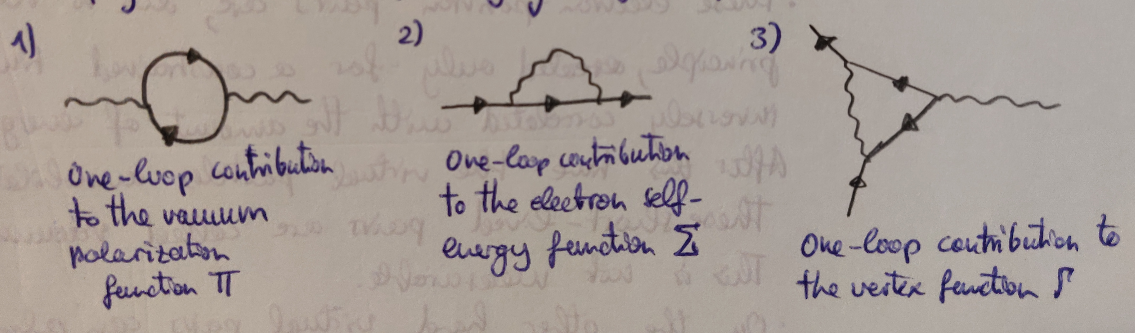
\includegraphics[width=0.7\linewidth]{gfx/DivergingIntegralsQED}
	\caption{\itshape Diverging integrals in QED appearing higher than tree level.}
	\label{fig:divergingintegralsqed}
\end{figure}
A theory is renormalizable, thus meaningful after renormalization, if the number of diverging diagrams is finite. The reason for this is that to get observables renormalized one needs a finite number of constants to maintain the predictive value of the theory untouched.
\subsubsection{The UV problems of QED}
Since $[e]=0$, QED is renormalizable with seven superficially (four actually) divergent diagrams. These are the following, where we used QED's SDOD \ref{eq:renormalizationSdodQED}.
\begin{enumerate}
	\item The vacuum energy $\feynmandiagram{b[blob]};$ with $D=4$.
	\item The photon propagator $\feynmandiagram[horizontal=a to b]{a--[boson] c[blob] -- [boson]b};$ with $D=2$; the electron propagator $\feynmandiagram[horizontal=a to b]{a --[fermion]c[blob] --[fermion]b};$ with $D=1$ and the $D=0$ vertex
	\begin{equation}
		\feynmandiagram[vertical=a to b]{a -- [boson] c [blob] -- d, c--b};.
	\end{equation}
	\item The 1-photon amplitude $\feynmandiagram[horizontal=a to b]{a[blob]--[boson]b};$ with $D=3$;
	\item The 3-photon amplitude with $D=1$
	\begin{equation}
	\feynmandiagram[vertical=a to b]{a -- [boson] c [blob] -- [boson] d, c --[boson] b};
	\end{equation}
	\item The 4-photon amplitude with $D=0$
	\begin{equation}
		\feynmandiagram[horizontal=a to b]{a--[boson] c [blob] -- [boson] d, e --[boson]c--[boson] b};
	\end{equation}
\end{enumerate}
Only the diagram from 1. and 2. are actually divergent. This is due to the symmetries at work in QED preventing some of QED's superficial divergencies:
\begin{enumerate}
	\item Discrete charge conjugation $j^{\mu} \rightarrow - j^{\mu}$ and $A^{\mu} \rightarrow - A^{\mu}$,
	\item Chiral symmetry (arises for $m=0$)
	\item Ward identity $k_{\mu}\mathcal{D}^{\mu} =0$ for a diagram $\mathcal{D}= \xi^{\mu} \mathcal{D}_{\mu}$ involving an external photon of momentum $k^{\mu} ( k^2 =0)$ and polarization $\xi^{\mu}$,
	\item Gauge symmetry $A^{\mu}(x) \rightarrow A^{\mu}(x) + \partial^{\mu} \alpha(x)$.
\end{enumerate}
The other diagrams vanish as follows:
\begin{enumerate}
	\item Amplitudes 3. and 4. vanish to all orders due to \emph{charge conservation}. A diagram with only an odd number of external photons vanishes, since each external photon couples via its current $j^{\mu}$.
	\item Diagram 5. is non-zero, but actually finite as a consequence of gauge symmetry, can be shown by exploiting the Ward identities.\\
	Note that this diagram is responsible for the non-linearity of QED due to the scattering of photons with each other induced by loop effects.\\
	$\rightarrow$ As far as the UV divergences are concerned it suffices to consider the diagram 2., because the contribution of 1. is easily absorbed into the vacuum energy term.
	\item By dimensional analysis it is found that all diagrams of 2. are logarithmically divergent.
\end{enumerate}

\subsubsection{Corrections to the fermion propagator}
Taking QED interactions into account the Feynman propagator $S_F(x-y)= \feynmandiagram[horizontal=a to b]{a [particle=y]-- [fermion] b [particle=x] };$ is corrected like
\begin{align}
\expval{\hat{T}\{\psi(x) \bar{\psi}(y)\}}{\Omega} &=
\feynmandiagram[horizontal=a to b]{a [particle=y] --c-- [fermion] b[particle=x]}; 
+ \feynmandiagram[horizontal=a to b]{a [particle=y]--c--[fermion] d--b [particle=x], c--[boson, half left] d };\nonumber \\
&	+\feynmandiagram[horizontal=a to b]{ a[particle=y] --c--[fermion] d -- e--f--[fermion] g--b[particle=x],
	c--[half left, boson]g, d -- [half left, boson ]f   } ; \\
&= 
\feynmandiagram[horizontal=a to b]{a[particle=y] -- c [blob] -- b [particle=x] };.
\end{align}

\begin{mybox}{Electron self-energy}
	Let 
	\begin{equation}
	\feynmandiagram[horizontal=a to b] {a [particle=A]--c [particle=$\left(1PI\right)$]--b[particle=B]  }; \equiv - i \sum(\slashed{p})_{AB}
	\end{equation}
	denote the amputated $1PI$ diagram. $\sum(\slashed{p})$ \emph{is called self-energy of the electron.}
	$\Rightarrow$ 
	\begin{align}
	\expval{\hat{T}\{\psi(x) \bar{\psi}(y) \}}{\Omega} &= \feynmandiagram[horizontal=a to b]{a[particle=y] --c--[fermion] b[particle=x] };
	+ \feynmandiagram[horizontal=a to b]{a--[fermion] c [particle=$\left(\sum\right)$]--[fermion] b  }; \nonumber \\
	&+ \feynmandiagram[horizontal=a to b]{a --[fermion]c[particle=$\left(\sum\right)$ ]--[fermion] d[particle=$\left(\sum\right)$] --[fermion]b  }; + \dots
	\end{align}
\end{mybox}
Where the full Feynman propagator for interacting QED theory takes the form (via Dyson resummation) 
\begin{equation}
\feynmandiagram[horizontal=a to b]{a [particle=y] --c [blob] -- b[particle=x]  };
= \int \frac{\md^4 p}{(2 \pi)^4} e^{-i p\cdot (x-y)} \; \frac{i}{\gamma \cdot p-m_0 - \sum(\slashed{p})+i \epsilon }.
\end{equation}



\subsubsection{Corrections to the photon propagator}
\begin{mybox}{Photon self-energy}
	The Fourier transform of the photon propagator, denoted by $\feynmandiagram[horizontal=a to b]{a --[boson] c [blob] --[boson]b};$, can be derived via Dyson resummation from the $1PI$ diagram 
	\begin{equation}
	\feynmandiagram[horizontal=a to b]{a[particle=$\mu$] -- [boson] c -- [boson] b[particle=$\nu$] };
	\equiv i \Pi^{\mu \nu} (q^2) = 
	\end{equation}
	which is the \emph{self-energy of the photon or vacuum polarization}.
\end{mybox}
Vacuum polarization describes the process in which a background electromagnetic field produces virtual electron-positron pairs that change the distribution of charges and currents that generated the original electromagnetic field. It is also referred to as the \emph{self-energy of the gauge boson(photon)}.\\
\\
These electron-positron pairs are, due to Heisenberg's uncertainty principle, created only for a constrained time, having duration inversely correlated with the amount of energy of the fluctuation. After this time the virtual particles annihilate each other. These short-lived pairs are called \emph{vacuum bubbles}. This is not measurable.\\
On the other hand virtual pairs can also occur as a photon progress, as seen in \ref{fig:divergingintegralsqed}; the effect on other processes is measurable.\\
$\Rightarrow$ Such charged pairs act as an electric dipole. In the presence of an electric field, e.g. the electromagnetic field around an electron, these particle-antiparticle pairs reposition themselves, thus partially counteracting the field.\\
The field therefore will be weaker than would be expected if the vacuum were completely empty. This reorientation of the short-lived particle-antiparticle pairs is referred to as  \emph{vacuum polarization}.

\subsubsection{Corrections to the interaction vertex}
\begin{mybox}{Vertex function}
	We define an effective vertex by summing up all loop-corrections. This is the \emph{vertex function} $\Gamma$, which describes the coupling between a photon and an electron beyond leading order, it is the one particle irreducible correlation function which involves $ \psi, \bar{\psi}$ and $A_{\mu}$:
	
\end{mybox}

\begin{figure}
	\centering
	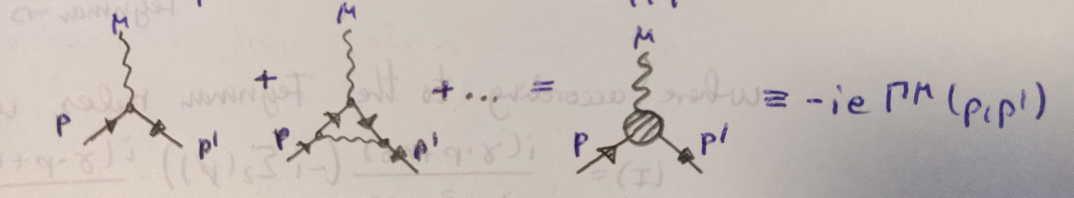
\includegraphics[width=0.7\linewidth]{gfx/VertexFunctionQED}
	\caption{\itshape Definition of the vertex function, summing up all loop corrections.}
	\label{fig:vertexfunctionqed}
\end{figure}
We will compute these corrections to 1-loop order. The diagrams will exhibit:
\begin{enumerate}
	\item Ultraviolet (UV) divergences from integrating the momenta of particles in the loop up to infinity.
	\item Infra-red (IR) divergences if the diagram contains massless particles (i.e. photons) running in the loop
\end{enumerate}
The general status of these divergences is as follows
\begin{enumerate}
	\item UV divergences require regularization of the integral and can be absorbed in a clever definition of the parameters via renormalization.
	\item IR divergences in loop-diagrams cancel if physical observables are computed.
\end{enumerate}



\subsection{Self-energy of the electron at 1-loop}
At 1-loop order the electron propagator takes the form 
\begin{equation}
\expval{\hat{T}\{\psi(x) \bar{\psi}(y)\}}{\Omega} =
\feynmandiagram[horizontal=a to b]{a [particle=y] -- [fermion] c-- b [particle=y]};
+ \underbrace{\feynmandiagram[horizontal=a to b]{a[particle=y] --[fermion] c-- b[particle=x]}; }_{\stackrel{Feynman}{\Rightarrow} \int \frac{\md^4 p}{(2 \pi)^4} e^{-i p(x-y) } \cdot (I) }
\end{equation}
where according to the Feynman rules we have
\begin{equation}
(I) = \frac{i(\gamma \cdot p +m_0)}{p^2-m^2_0+i \epsilon} \left(-i \sum_2(\slashed{p})\right) \frac{i(\gamma \cdot p+m_0)}{p^2-m^2_0 +i\epsilon}.
\end{equation}
$\Rightarrow$ The amputated 1-loop contribution corresponds to omitting the two outer fermion propagators and is thus given by:
\begin{equation}
-i \sum_2(\slashed{p}) = (-i e)^2 \int \frac{\md^4 k}{(2 \pi)^4} \gamma^{\mu} \frac{i(\slashed{k}+m_0)}{k^2-m^2_0+i \epsilon} \gamma^{\nu} \frac{(-i \eta_{\mu \nu})}{(p-k)^2 + i \epsilon}.
\end{equation}
This integral has a IR-divergence near $k=0$ if $p\rightarrow0$. We will introduce a fictitious small photon mass $\mu$ to regulate the IR divergence:
\begin{equation}
\Rightarrow i \sum_2(\slashed{p}) = (-ie)^2 \int \frac{\md^4 k}{(2 \pi)^4} \gamma^{\mu} \frac{i (\slashed{k}+m_0)}{k^2-m^2_0 +i \epsilon} \gamma_{\mu} \frac{-i}{(p-k)^2-\mu^2+i \epsilon}.
\end{equation}
The evaluation of such typical momentum integrals proceeds as detailed in \ref{subsubsec:renormalizationDimReg}.

\subsubsection{Explicit discussion of renormalized QED}
We have four counterterms $\delta_{1,2,3,m}$ and four renormalization conditions at (at $1$-loop level). Applying the latter ones will thus give us the exact expressions of the counterterms.\\
QED is a gauge theory and therefore $\mL$ has to be gauge-invariant. We can use this to determine identities:\\
Applying a gauge shift we find that $\mL^\prime_{QED}=\mL_{QED}$ for $Z_1=Z_2$ (which holds to all orders in perturbation theory).\\
We have the renormalization conditions:
\begin{align}
	\Sigma(\slashed{p})|_{\slashed{p}=m} &=0 \\
	\Leftrightarrow\; &\text{set physical mass as pole mass}: \frac{i Z_2}{p^2-m^2-i\Sigma}\nonumber\\
	\frac{\md}{\md \slashed{p}} \Sigma(\slashed{p}) |_{\slashed{p}=m} &= 0,\\
	\Leftrightarrow &\text{residue is }1.\nonumber\\
	-ie \Gamma^\mu(p+q,p) |_{q^2=0} &=0,\\
	\Pi(q^2)|_{q^2=0} &=0,
\end{align}
where $\Sigma(\slashed{p})$ is the mass operator (also sometimes referred to as self-energy), $\Pi(q ^2)$ is the polarization operator (thus the gauge boson self-energy, i.e. photon's) and $\Gamma^\mu(p^\prime,p)$ is the vertex correction (quantum corrections to the interaction term describing gauge boson and fermion interactions).\\
At $1$-loop
\begin{enumerate}
	\item Amputated self-energy of the electron (i.e. fermion self-energy) 
	\begin{equation}
		\feynmandiagram{a--c[particle=$1PI$]--b}; = -i \Sigma(\slashed{p})|_{1-loop} = \feynmandiagram[horizontal=v to w]{a--v--[fermion] w--b, v--[half left, boson] w};+
		\underbrace{\feynmandiagram{a--v[crossed dot]--b};}_{i(\slashed{p}\delta_2-\delta_m)}.
	\end{equation}
	\item Amputated self-energy of the photon (i.e. gauge boson self-energy)
	\begin{equation}
		\feynmandiagram{a[particle=$\mu$] --[boson] v [particle=$1PI$] -- [boson] b[particle=$\nu$]}; = i \Pi\munu(q^2)|_{1-loop} = \feynmandiagram[horizontal=v to w]{a[particle=$\mu$] --[boson] v--[half left, edge label=$q$] w--b[particle=$\nu$], w--[half left] v}; +
		\feynmandiagram{a[particle=$\mu$] --[boson] v[crossed dot] --[boson] b [particle=$\nu$]};.
	\end{equation}
	\item Vertex (not amputated):
	\begin{align}
	&\feynmandiagram[horizontal=v to w]{a --[fermion, momentum=\(p\)] v[particle=$\left(1PI\right)$] --[boson, edge label=$k$] h--[boson] w [particle=\mu], v --[fermion, momentum=\(q\)]b }; = -ie \Gamma^\mu(q,p,k) |_{1-loop} \\
	&= \feynmandiagram{a--v--[boson]b[particle=$\mu$], c--v};
	+\feynmandiagram[vertical=a to b]{a--x--v--[boson] c[particle=$\mu$], b--y--v, y--[boson] x}; 
	+\feynmandiagram{a--v[crossed dot] --[boson] b[particle=$\mu$], c--v};.\nonumber
	\end{align}
\end{enumerate}
Now we apply renormalization conditions on these operators in order to have an algebraic system of equations for the counterterms, which can be solved by consecutive elimination since there is one renormalization condition per counterterm.\\
If we plug in these exact expressions into $\mL_{QED}$, we find that all divergences vanish, such that we can predict experiment or, the other way around, take physical parameters to compute bare parameters.
\paragraph{Note}
The Ward-Takahashi identity shows $\delta_1=\delta_2$.
\subsubsection{Physical discussion of renormalized QED}
A scale for the system only enters through the counterterms, by imposing renormalization conditions. From the above and $\delta_1=\delta_2$, one can find the QED 1-loop $\beta$ function
\begin{equation}
	\beta^{1-loop}_e(\mu)= \mu \frac{\partial}{\partial \mu} \left(-e \delta_1+e\delta_2 + e \half \delta_3\right)= \mu \frac{\partial}{\partial \mu} \left(e \half \delta_3\right).
\end{equation}
The given expressions of $\delta_1,\delta_2$ and $\delta_3$ are derived in the case of \emph{on-shell} renormalization at $p^2=m^2$ (where $m$ is the physical mass of the electron). Thus, in this case "$m$" identifies the mass scale and we can set $\mu=m$, i.e.
\begin{equation}
	\beta_e(\mu) |_{1-loop, QED} = \frac{e^3}{12 \pi^2}.
\end{equation}
Identifying $\alpha =\frac{e^2}{4 \pi}$, we find
\begin{equation}
	\alpha(\mu) = \frac{\alpha^*}{1-\frac{2}{3 \pi} \alpha^* \ln(\frac{\mu}{\mu^*}) }\quad \alpha^* \equiv \alpha(\mu^*).
\end{equation}
Thus, the QED coupling diverges at the \emph{Landau pole} $\mu = \mu^* \exp(\frac{3\pi}{2 \alpha^*})$, but perturbation theory becomes unapplicable already at $\mu_0$ such that $\alpha(\mu_0)=1$, i.e. 
\begin{equation*}
	\mu_0 = \mu^* \exp \left[\frac{3\pi}{2} \left(\frac{1}{\alpha^*} -1\right)\right].
\end{equation*}
The solution was to realize that the quantities initially appearing in the theory's formula (e.g. $\mL$), representing such things as the electron's electric charge and mass, as well as the normalization of the quantum fields themselves, did not actually correspond to the physical constant measured in the laboratory. They were bare quantities that did not take into acount the contribution of virtual-particle loop effects to the physical constants themselves. In general, these effects would be just as divergent as the amplitudes under consideration in the first place; so finite measured quantities would, in general, imply divergent bare quantities.\\
To make contact with reality, then, the formulae would have to be rewritten in terms of measurable, renormalized quantities. The charge of the electron, say, would be defined in terms of a quantity measured at a specific kinematic renormalization point or subtraction point (which will generally have a characteristic energy, called \emph{renormalization scale} or simply the energy scale). The parts of the Lagrangian left over, involving the remaining portions of the bare quantities, could then be reinterpreted as counterterms, involved in divergent diagrams exactly canceling out the troublesome divergences for other diagrams.\\
In QFT, and especially in QED, the interacting theory leads to infinite quantities that have to be absorbed in a renormalization procedure, in order to be able to predict measurable quantities. The renormalization scheme can depend on the type of particle that are being considered. For particles that can travel asymptotically large distances, or for a low energy process, the $1)$ \emph{on-shell} or \emph{physical scheme} is appropriate
\begin{enumerate}
	\item The parameters of a theory are, for e.g. QED, $\psi, A, m$ and $e$. These quantities happen to be infinite due to loop corrections. One can derive renormalized quantities, which will be finite and observable, via e.g. wavefunction renormalization. The $\delta_i$ are called \emph{counterterms}, they are supposed to be small in $e$.\\
	\emph{Renormalization conditions} are then a set of rules that describe what part of the divergences should be in the renormalized quantities and what parts should be in the counterterms.\\
	In the interacting QED theory, two quantities are introduced. First, the \emph{renormalized mass} $m_r$ has been defined as the pole in the Fourier transform of the Feynman propagator. This is the main prescription of the \textbf{on-shell renormalization scheme} (there is no need to introduce other mass scales like in the MS scheme). This means that $m_r$ and $Z_2$ can be defined as a series in $e$ if this parameter is small enough.\\
	The modification to the Feynman propagator ($m\rightarrow m_r$, $1\rightarrow Z_2$) are summed up in the fermion self-energy $\Sigma(p)$
	\begin{equation}
		\bra{\Omega}T\psi(x) \bar{\psi}(x)\ket{\Omega} = \int \frac{\md^4 p}{(2 \pi)^4} \frac{iZ_2 e^{-ipx}}{\slashed{p} -m_r+i\epsilon} = \int \frac{\md^4 p}{(2 \pi)^4} \frac{i e^{-i p x}}{\slashed{p} - m-\Sigma(p) +i\epsilon}.
	\end{equation}
	These corrections are often divergent because they contain loops. By identifying the two expressions of the correlation function up to a certain order in $e$, the counterterms can be defined, and they are going to absorb the divergent contributions of the corrections to the fermion propagator. Thus, the renormalized quantities, such as $m_r$, will remain finite and will be the quantities measured in experiments.
	\item \begin{mybox}{MS-Scheme}
	The MS (minimal subtraction)-scheme contains isolating poles via dimensional regularization and to absorb only the divergent part of the radiative corrections into the counterterms, i.e. we only subtract $\frac{1}{\epsilon}$ terms.
	\end{mybox}
\item \begin{mybox}{$\bar{MS}$-Scheme}
	This modified MS-Scheme contains isolating poles via dim. reg. and absorbing the complete radiative correction 
	\bse 
	\frac{1}{\epsilon} - \gamma_{E} + \ln(4\pi) 
	\ese 
	into the counterterms.
\end{mybox}
\end{enumerate}


\subsection{Second example for on-shell renormalization --phi 4 theory renormalized}
\label{subsec:renormalizationPhi4}
$\phi^4$ theory is perturbatively renormalizable in $d=4$ because 
\begin{equation}
[\lambda]=0.
\end{equation}
\subsubsection{Superficially divergent amplitudes in $d=4$}
Superficial degree of divergence is 
\begin{equation}
D=4-E \Rightarrow\; E\leq 4 \text{ are divergent amplitudes},
\end{equation}
such that amplitudes with $E\leq 4$ are superficially divergent.
\begin{align}
	&E=0 \Rightarrow D=4: \quad (\text{vacuum energy})\\
	&[E=1 \Rightarrow D=3 \quad (\text{tadpole})]\\
	&E=2 \Rightarrow D=2: \quad D_F(p^2) \; (\text{propagator})\\
	&[E=3 \Rightarrow D=1 \quad (\phi^3 \text{ vertex})]\\
	&E=4 \Rightarrow D=0: \quad \mM_4(s,t,u) (\phi^4 \text{ vertex}).
\end{align}
Amplitudes with odd numbers of $\phi$ vanish by $Z_2$ symmetry $\phi \rightarrow - \phi$ and eliminate the divergence of $E=1$ and $E=3$ so we are left with $3$ divergent amplitudes.
\subsubsection{Renormalization conditions and renormalized perturbation theory}

\begin{mybox}{Example of how to renormalize via counterterms}
	The renormalization conditions are
	\begin{align}
		D_F(p^2) = \frac{i}{p^2-m^2-M^2(p^2)} &\stackrel{!}{=} \frac{i}{p^2-m^2} + (\text{regular})\\
		\mM_4(4m^2,0,0) \stackrel{!}{=} -i\lambda.
	\end{align}
	Introduce the notation
	\begin{equation}
	\phi := \frac{\phi_0}{\sqrt{Z}},\; \delta_\phi:= Z-1,\; \delta_m:= m^2_0 Z-m^2,\; \delta_\lambda:= \lambda_0 Z^2-\lambda
	\end{equation}
	to rewrite the Lagrangian in terms of a renormalized Lagrangian $\mL_r$ and counter terms
	\begin{equation}
	\mL = \mL_r+\frac{\delta_\phi}{2} (\partial \phi)^2 - \frac{\delta_m}{2} \phi^2 - \frac{\delta_\lambda}{4!} \phi^4
	\end{equation}
	such that we get new vertices at order $\lambda$:
	\begin{align}
		\expval{ \prod_{i=1}^{2}\phi(x_i) \int \md^4  \left(\frac{\delta_\phi}{2} (\partial \phi)^2 - \frac{\delta_m}{2} \phi^2\right)} &\leftrightarrow i(p^2\delta_\phi -\delta_m) \\
		\expval{ \prod_{i=1}^4 \phi(x_i) \int \md^4x \frac{-\delta_\lambda}{4!}\phi^4 (x) } &\leftrightarrow -i \delta_{\lambda}.
	\end{align}
	Note that the proapgator renormalization condition in terms of scalar self-energy $M^2(p^2)$ is
	\begin{equation}
	M^2(m^2) \stackrel{!}{=}0 \text{  and  } \frac{\md}{\md p^2}M^2(m^2) \stackrel{!}{=}0.
	\end{equation}
\end{mybox}
Introduction of counterterms explicitly:
\begin{align*}
	\mL &= \half (\partial \phi_0)^2 -\half m^2_0 \phi^2_0 - \frac{\lambda_0}{4!} \phi^4 \\
	&= \half \partial(\sqrt{Z}\phi)^2-\half m^2_0(\sqrt{Z}\phi)^2 - \frac{\lambda_0}{4!}(\sqrt{Z} \phi)^4 \\
	&= \half Z(\partial \phi)^2 - \half Z m^2_0 \phi^2 - \frac{\lambda_0}{4!} Z^2 \phi^4 \\
	&= [\half Z(\partial \phi)^2+\half (\partial \phi)^2-\half (\partial \phi)^2] \\
	&-[\half Zm^2_0 \phi^2+\half m^2 \phi^2-\half m^2\phi^2] \\
	&- [\frac{\lambda_0}{4!}Z^2\phi^4 + \frac{\lambda}{4!} \phi^4-\frac{\lambda}{4!}\phi^4 ]\\
	&= \mL_r + [\half Z(\partial \phi)^2-\half(\partial \phi)^2]\\
	&-[\half Z m^2_0 \phi^2-\half m^2\phi^2] - [\frac{\lambda_0}{4!} Z^2 \phi^4 -\frac{\lambda}{4!} \phi^4] \\
	&=\mL_r + \half [Z-1] (\partial \phi)^2 - \half [Zm^2_0-m^2] \phi^2-\frac{1}{4!} [\lambda_0 Z^2-\lambda] \phi^4\\
	&= \mL_r+ \frac{\delta_\phi}{2} (\partial \phi)^2 -\frac{\delta_m}{2} \phi^2 - \frac{\delta_\lambda}{4!}\phi^4 \qquad \blacksquare
\end{align*}
\subsubsection{Explicit renormalization analysis of $\phi^4$}
\label{subsubsec:phifourrenormalization}
We have, as exemplified above
\begin{align*}
	\mL_{\phi^4} &= \half (\partial \phi_0)^2-\frac{m^2_0}{2} -\frac{\lambda_0}{4!} \phi^4_0 \\
	&= \half (\partial \phi)^2-\frac{m^2}{2}\phi^2-\frac{\lambda}{4!}\phi^4 + \frac{\delta_Z}{2} (\partial \phi)^2 -\frac{\delta_m}{2} \phi^2 -\frac{\delta_\lambda}{4!} \phi^4\\
	&=\mL_r +  \frac{\delta_Z}{2} (\partial \phi)^2 -\frac{\delta_m}{2} \phi^2 -\frac{\delta_\lambda}{4!} \phi^4 
\end{align*}
where we split the divergent Lagrangian into two contributions. The first only contains finite so-called \emph{renormalized quantities} with values as they would be measured in experiment. The second part absorbs all divergences in so-called \emph{counterterms}. These are for $\phi^4$:
\begin{align*}
	\phi &= \phi_0 Z^{-\half} \text{ wavefunction renormalization}\\
	\feynmandiagram{a--[fermion]b}; &= \frac{i}{p^2-m^2+i \epsilon},\\
	\feynmandiagram[horizontal=a to b]{a--[fermion] c [crossed dot] --[fermion] b};&= i (p^2 \delta_Z-\delta_m),\\
	\feynmandiagram{a--v[dot]--b, c--v--d};&=- i \lambda,\\
	\feynmandiagram{a--v[crossed dot] --b, c--v--d}; &=-i \delta_\lambda.
\end{align*}
In this theory we have
\begin{equation}
D=4L-2P,\; L=P-V+1 \; \text{use Euler } 4 V=2 P+E \; \Rightarrow D=4-E.
\end{equation}
Thus, $\lambda \phi^4$ theory is renormalizable, also seen by $[\lambda]=0$ vanishing mass-dimension.\\
The superficially divergent diagrams are
\begin{enumerate}
	\item $\feynmandiagram{a[blob]};\quad D=4$,
	\item $\feynmandiagram{a--b[blob]}; \quad D=3$,
	\item $\feynmandiagram{a--c[blob]--b};\quad D=2$,
	\item $\feynmandiagram{a--c[blob]--b, d--c}; \quad D=1$
	\item $\feynmandiagram{a--v[blob]--b, d--v--e};\quad D=0$.
\end{enumerate}
Since $\mL_{\phi^4}$ is invariant under Paritiy transformation (\textbf{always check for symmetries !}), all diagrams with an odd number of external lines vanish: $2\&4)=0$. \\
Why are we tasked with renormalizing the propagator and the vertex ?\\
The vacuum diagram can be trivially absorbed in the vacuum energy density $V_0$, an additional degree of freedom of any Lagrangian, which we did not write down explicitly, since the absolute energy scale is meaningless in a theory without gravity. Thus, propagator and vertex are the only fundamental divergences in $\phi^4$-theory . All others are due to diagrams containing those two as subdiagrams.\\
\\
$s,t,u$-channel have identical contributions with $s=p^2=(p_1+p_2)^2$, $u=p^2=(p_1-p_4)^2$, $t=p^2=(p_1-p_3)^2$
\begin{align}
	(-i \lambda)^2 i V(p^2) &:= \frac{(-i \lambda)^2}{2} \int \frac{\md^d k}{(2 \pi)^d} \frac{i}{k^2-m^2+i\epsilon} \frac{i}{(p+k)^2-m^2+i\epsilon} \\
	&\equiv \feynmandiagram [layered layout, horizontal=i_1 to f_1] [edges=fermion] {
		{i1, i2} -- a -- [half left, momentum=\(k\)] b -- [half left, momentum=\(k-p\)] a,
		b -- {f1, f2},
	};;.
\end{align}
Now we fix some energy scale $s_0,u_0,t_0$ and insert it into the $1$-loop amplitude to remove the divergences.
\todo{Finish this treatment}
\\
\\
If we were to consider the propagator to second loop order, we would have to look at
\begin{align}
	-i M^2(p^2) |_{\mO(\lambda^2)} &= \feynmandiagram{a -- c [particle=$1PI$]--b}; \\
	&= \feynmandiagram{a--v--b,v--[loop] v};+ \feynmandiagram[horizontal=v to w]{a--v--w--v, v--[half left] w, w--[half left] v, w--b}; \\
	&+\feynmandiagram[horizontal=a to b]{a --v[crossed dot] --b, v--[half left,loop] v};+\feynmandiagram{a--v[crossed dot]--b[particle=$\delta^{1-loop}_Z$]}; 
	\\
	&+ \feynmandiagram{a--v[crossed dot]--b[ particle=$\delta^{2-loop}_Z$]};. 
\end{align}
In general, one can simply write down the diagrams via the Feynman rules and then impose the renormalization conditions on them to identify the counter-terms From this, one can already extract the form of the propagator or transition amplitude. Afterwards, one can do the dimensional reg. calculation in order to explicitly find divergences and hide it in the counterterms.
\\
\\
Note that we can write 
\begin{equation}
\feynmandiagram[horizontal=a to b]{a--v[crossed dot] --b, v--[half left] v};= \left[	\feynmandiagram[horizontal=a to b]{a--v --b, v--[loop] v};\right]_{\lambda \rightarrow \delta_\lambda}.
\end{equation}


\subsection{Third example of on-shell renormalization - YM renormalized}
\label{subsec:renormalizationYM}
Strictly speaking, the renormalization of YM should happen before QCD as QCD is only a special case of YM theory. As this treatment is only very crude, it is has more pedagogical value for the reader to follow the renormalization of QCD to get a sense of the logic behind on-shell renormalization. If this is a first read through, I would therefore recommend to jump to \ref{subsec:renormalizationqcd} to get the idea and come back to \ref{subsec:renormalizationYM} after that. This treatment is more a collection of important results.\\
YM theory is power-counting renormalizable since $[g]=0$.\\
We start from the bare gauge-fixed Lagrangian
\begin{align*}
	\mL &= - \frac{1}{4} \left(\partial_\mu A^a_{0\;\nu} - \partial_\nu A^a_{0 \; \mu} \right)^2 - \frac{1}{2 \xi_0} (\partial A^a_0)^2 + \bar{\psi}_0 (i \slashed{\partial} - m_0) \psi_0 \\
	& - \bar{c}_c \partial_\mu \partial^\mu c_0 - g_0 A_{0\mu} \bar{\psi}_0 \gamma^\mu T^a \psi_0 + g_0 f^{abc} (\partial_\mu A^a_{0\nu}) A^{b\mu}_0 A^{c \nu}_0 \\
	&-\frac{1}{4} g^2_0 f^{abc} f^{ade} A^{\mu b}_0 A^{\nu c}_0 A^d_{\mu 0} A^e_{\nu 0} + g_0 \bar{c}_0 f^{abc} \partial^\mu A^b_{0 \mu} c^c_0
\end{align*}
and we perform field strength renormalizations
\begin{equation}
A_0 = \sqrt{Z_3}A, \; \xi_0=Z_3 \xi, \; \psi_0= \sqrt{Z_2}\psi, \; \stackrel{(-)}{c}_0 = \sqrt{Z^c_2} \stackrel{(-)}{c}.
\end{equation}
This gives eight counterterms - not all independent:
\begin{align*}
	\delta_2 &=Z_2 -1, \; \delta_3 = Z_3-1, \; \delta^{(c)} = Z^{(c)}_2 -1, \; \delta_m = Z_2 m_0 -m,\\
	\delta_1 &= \frac{g_0}{g} Z_2 \sqrt{Z_3}-1, \delta^{cubic}_1 = \frac{g_0}{g} Z^{3/2}_3-1,\\
	\delta^{quartic}_1 &= \frac{g_0}{g}Z^2_3-1, \; \delta^{(c)}_1 = \frac{g_0}{g} Z^c_2 \sqrt{Z_3}-1.
\end{align*}
Note: Due to renormalization of $\xi_0$, the kinetic counterterm for $A_\mu$ becomes independent of $\xi$
\begin{equation*}
	-\frac{1}{4} \delta_3 ( \partial_\mu A_\nu - \partial_\nu A_\mu)^2.
\end{equation*}
Thus, among others, we have the counterterms
\begin{align}
	\feynmandiagram[horizontal=a to b]{a [particle=$A$] -- [gluon] c [crossed dot] --[gluon] b [particle=$b$]};
	&= -i (k^2 \eta^{\mu \nu} - k^\mu k^\nu) \delta^{ab} \delta_3 \\
	\feynmandiagram[horizontal=a to b]{a [particle=$i$] --[anti fermion] c [crossed dot] -- [anti fermion] b [particle=$j$]};
	&= i \gamma^\mu p_\mu \delta_2 \delta_{ij} \\
	\feynmandiagram[horizontal=a to b]{a -- [fermion] v [crossed dot] -- [anti fermion] b, c [particle=${(\mu,a)}$] --[boson] v};
	&= -ig T^a \gamma^\mu \delta_1
\end{align}
and in addition those for $A^3,A^4, \bar{c} A c+\bar{c} c$ $\& \psi$-mass.+
\\
\\
Our Aim is to extract the $1$-loop $\beta$-function for $g$.\\
Since $\beta(g)$ is sensitive only to UV-divergences, we can henceforth set $m=0$. As in QED, we extract $\beta(g)$ from the Callen-Symancyk equation for the $3$-point function $\expval{A\bar{\psi} \psi}$ as
\begin{equation}
\beta(g) = g \mu \frac{\partial}{\partial \mu} \left(-\delta_1 + \delta_2 + \half \delta_3\right) \quad \text{at $1$-loop}.
\end{equation}
We therefore only need the $mu$-dependence of $\delta_1,\delta_2,\delta_3$. We will see that after cancellations all divergences are of the form 
$\frac{\Gamma(2-\frac{\md}{2})}{\Delta^{2-\frac{\md}{2}} }$ in dimensional regularization with $\Delta$ some $p^2$-invariant. We can identify
\begin{equation}
\mu^2 = \Delta
\end{equation}
by choice of renormalization conditions and extract only the divergences of $\delta_i$ for $\beta(g)$.



\subsubsection{Preliminaries in Group Theory}
Given a representation $R$ with $T^a_R \equiv (T^a_R)_{ij}$, $i,j=1,\dots,\dim R$, i.e. a matrix representation, of a Lie algebra $Lie(H)$ with dimension $\dim H$, the \emph{second Casimir} $C_2(R)$ is defined via 
\begin{equation}
\sum_a T^a_R T^a_R = T^a_R T^a_R= C_2(R) \cdot \mI.
\end{equation}
If we normalize the $T^a_R$ such that
\begin{equation}
\tr T^a_R T^b_R = \underbrace{C(R)}_{\text{normalization group factor}} \delta^{ab}
\end{equation}
then
\begin{equation}
\dim(R) C_2 (R) = C(R) \cdot \dim(H).
\end{equation}
Consider the examples
\begin{enumerate}
	\item Let $R=f$ be the fundamental representation of $SU(N)$ normalized such that\begin{equation}
	\tr(T^a_f T^b_f) = \half \delta^{ab} \quad \Rightarrow \quad C(f) = \half.
	\end{equation}
	Then 
	\begin{equation}
	C_2(f) = \half \frac{\dim(SU(N)) }{\dim(f)} = \half \frac{N^2-1}{N}.
	\end{equation}
	\item Let $R=Ad$ be the adjoint representation of $H$, defined such that 
	\begin{equation}
	(T^b_{Ad})_{ac} = i f^{abc} \quad \Rightarrow \quad C(H) := C(Ad)
	\end{equation}
	computable via
	\begin{align*}
		C(H)\delta^{ab} &= \tr(T^a_{Ad} T^b_{Ad})= -f^{dac} f^{cbd},\quad C(H) \delta^{ab} = f^{acd} f^{bcd} \\
		C_2(H) \delta^{ab} &= (T^a_{Ad})_{bc} (T^a_{Ad})_{cd} = f^{cab} f^{cae} \\
		\Rightarrow \quad C(H) & = C_2(H),
	\end{align*}
	also follows since $\dim(Ad)=\dim(H)$. For example, $H=SU(N)$ gives us 
	\begin{equation*}
		C(SU(N)) = N.
	\end{equation*}
\end{enumerate}



\subsubsection{Computation of $\delta_3$}
\begin{figure}[h!]
	\centering
	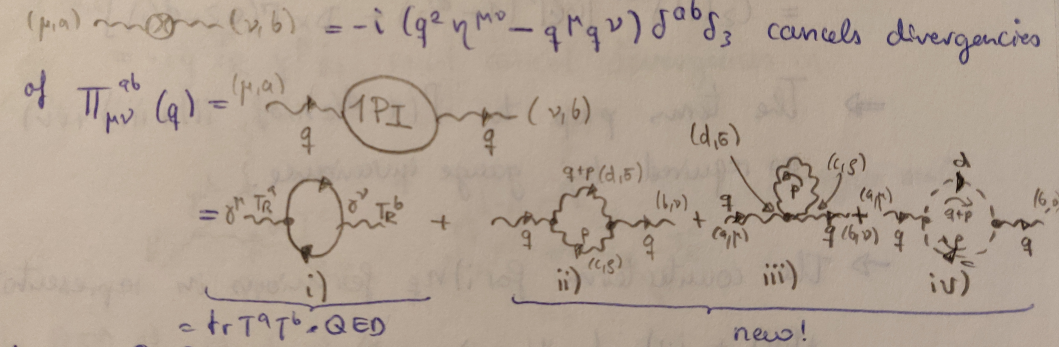
\includegraphics[width=0.5\linewidth]{gfx/YMpictures/YMselfenergy}
	\caption{YM self-energy renormalization}
	\label{fig:ymselfenergy}
\end{figure}
As in QED, \begin{equation}
q^\mu \Pi\munu(q)=0,
\end{equation}
which is a consequence of the Slavnov-Taylor identities. So we have
\begin{equation*}
	\Pi\munu(q)=i (q^2 \eta^{\mu \nu} - q^\mu q^\nu) \Pi(q^2).
\end{equation*}
Thus, compute the four diagrams $i)-iv)$ to find $\delta_3$:
\begin{enumerate}
	\item[i)] Choosing $\Delta:= -x(1-x)q^2$ with renormalization scale $\mu$, we find
	\begin{equation}
	\delta_3 |_{i)} = -\frac{g^2}{(4 \pi)^2} \frac{4}{3} C(R) \frac{\Gamma(2-\frac{\md}{2})}{(\mu^2)^{2-\frac{\md}{2}}}
	\end{equation}
	for a fermion in representation $R$.\\
	\\
	Note that the pure YM diagrams $ii)-iv)$ (pure in the sense that they do not appear in QED) are computed in Feynman gauge $\xi=1$.
	\item[ii)] Contains two types of divergences, via dimensional Regularization:
	\begin{enumerate}
		\item $\Gamma(2-\frac{\md}{2})\times \dots \leftrightarrow$ corresponds to logarithmic divergences in $\md=4$.
		\item $\Gamma(1-\frac{\md}{2})\times \dots \leftrightarrow$ corresponds to logarithmic divergence in $\md=2$, i.e. $\int \frac{\md^{\md} p}{(p^2)}$ and thus a quadratic divergence in $\md=4$.
	\end{enumerate}
	A quadratic divergence would indicate a renormalization of the gauge boson mass, which is forbidden by gauge invariance. This term must hence cancel against other contributions.
	\item[iii)]
	\begin{equation}
	iii)= \left[A \cdot \Gamma(1-\frac{\md}{2}) + B\cdot \Gamma(2-\frac{\md}{2}) \right] C_2(H) \delta^{ab} 
	\end{equation}
	\item[iv)]
	We get a $(-1)$ sign from Grassman fields in loop
	\begin{align}
		iv)&= (-1) \int \frac{\md^4p}{(2 \pi)^4} \frac{i}{p^2} \frac{i}{(p+q)^2} g^2 f^{dac} (p+q)^\mu f^{cbd} p^\nu \nonumber \\
		&= C_2(H) \delta^{ab} \left[C \cdot \Gamma(1-\frac{\md}{2}) + D\cdot \Gamma(2-\frac{\md}{2})\right].
	\end{align}
\end{enumerate}
The terms proportional to $\Gamma(1-\frac{\md}{2})$ of $ii)+iii)+iv)$ precisely cancel - as required by gauge invariance.
\\
Thus, the counterterm for $1)$ $n_f$ fermions in Representation $R_f+2)+3)+4)$ (with $\Delta= \mu^2$) is
\begin{equation}
\delta_3 = \frac{g^2}{(4 \pi)^2} \frac{\Gamma(2-\frac{\md}{2})}{(\mu^2)^{2-\frac{\md}{2}}} \left[\frac{5}{3} C_2(H) - \frac{4}{3} n_f C(R_f)\right].
\end{equation}



\subsubsection{Computation of $\delta_2$}

\begin{figure}[h!]
	\centering
	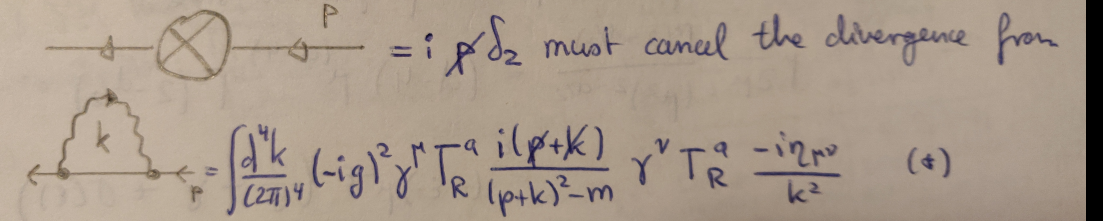
\includegraphics[width=0.7\linewidth]{gfx/YMpictures/YMoneLoopDelta2}
	\caption{}
	\label{fig:ymoneloopdelta2}
\end{figure}
Since we only need the UV divergences, we set again $m=0$.
\\The group theory factor is $T^a_R T^a_R = C_2(R) \cdot \mI$, thus
\begin{align}
	\ref{fig:ymoneloopdelta2} &= C_2(R)\mI  \times \left(\feynmandiagram[horizontal=a to b]{a--c--d--b, c--[boson, half left]d};\right)|_{QED} \\
	&= C_2(R) \frac{i g^2}{(4 \pi)^{\frac{\md}{2}} } \slashed{p} \int_0^1 \md x (1-x)(\md -2 ) \frac{\Gamma(2-\frac{\md}{2})}{\Delta^{2-\frac{\md}{2}}}
\end{align}
with $\Delta=-x(1-x)p^2$.\\ 
Identifying $\Delta=\mu^2$ yields
\begin{equation}
\delta_2 = - \frac{g^2}{(4 \pi)^2} \frac{\Gamma(2-\frac{\md}{2})}{(\mu^2)^{2-\frac{\md}{2}} } C_2(R).
\end{equation}


\subsubsection{Computation of $\delta_1$}
\begin{figure}[h!]
	\centering
	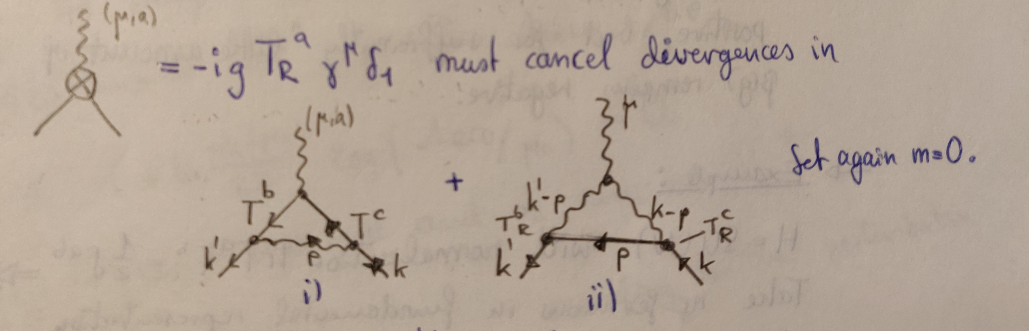
\includegraphics[width=0.7\linewidth]{gfx/YMpictures/YMoneLoopDeltaOne}
	\caption{}
	\label{fig:ymoneloopdeltaone}
\end{figure}
Consider the two separate diagrams individually
\begin{enumerate}
	\item[i)] In QED the Ward identities imply $\delta_1 |_{QED} = \delta_2|_{QED}$. We can factorize the diagram into contributions from YM and QED similar interactions like the following with this identity
	\begin{equation}
	\delta_1 |_{i)} = \underbrace{- \frac{g^2}{(4 \pi)^2} \frac{\Gamma(2-\frac{\md}{2})}{(\mu^2)^{2-\frac{\md}{2}} }}_{= T^a_R \cdot ({i)}_{QED})} \left(C_2(R)-\half C_2(H)\right),
	\end{equation}
	where we used the results from our QED calculations and just included the group theory factor..
	\item[ii)] Applying the same logic here, we find
	\begin{equation}
	\delta_1 |_{ii)} = -\frac{g^2}{(4 \pi)^2} \frac{\Gamma(2-\frac{\md}{2})}{(\mu^2)^{2-\frac{\md}{2}} } \frac{3}{2} C_2(H).
	\end{equation}
\end{enumerate}
Altogether
\begin{equation}
\delta_1 = - \frac{g^2}{(4 \pi)^2} \frac{\Gamma(2-\frac{\md}{2})}{(\mu^2)^{2-\frac{\md}{2}}} \left[C_2(R)+C_2(H)\right].
\end{equation}

\subsubsection{YM  $\beta$-function at $1$-loop in $g$}
The final result is found by noting that the divergencies vanish for the computation of the $\beta$-function since
\begin{align*}
	\mu \frac{\partial}{\partial \mu} \frac{\Gamma(2 -\frac{\md}{2})}{(\mu^2)^{2-\frac{\md}{2}} } &= (\md -4) \mu^{(\md-4)} \Gamma(2-\frac{\md}{2}) \\
	&\stackrel{\md=4-\epsilon}{=} (-\epsilon) \mu^{-\epsilon} \left(\frac{2}{\epsilon} -\gamma + \mO(\epsilon)\right) \\
	&\stackrel{\epsilon\rightarrow 0}{=} -2.
\end{align*}
\begin{mybox}{YM $\beta$ function to leading order in $\md=4$}
	\begin{equation}
	\label{eq:betafunctionYangMills}
	\beta^{(1)}_{YM}(g) = - \frac{g^3}{(4 \pi)^2} \left[\frac{11}{3} C_2(H) - \frac{4}{3} n_f C(R_f)\right].
	\end{equation}
\end{mybox}



\subsection{Fourth example for On-shell renormalization -- QCD renormalized}
\label{subsec:renormalizationqcd}
\subsubsection{Superficially divergent vertex functions in QCD}
Again, the logic is to renormalize divergent $1PI$ graphs. To find these we employ again power-counting via SDOD \ref{eq:renormalizationSdodQCD} and will look at the explicit symmetries of the theory to nail down the graphs which are actually divergent.
\begin{enumerate}
\item \feynmandiagram[horizontal=a to b]{a--[gluon] v1 --[gluon] v2 [particle=$(1PI)$] --[gluon] v3 --[gluon] b }; \quad D=2.
\item \feynmandiagram[horizontal=a to b]{a--[fermion] v1 --[fermion] v2 [particle=$(1PI)$] --[fermion] v3 --[fermion] b }; \quad D=1.
\item \feynmandiagram[horizontal=a to b]{a--[scalar] v1 --[scalar] v2 [particle=$(1PI)$] --[scalar] v3 --[scalar] b }; \quad D=2.
\item \feynmandiagram[horizontal=a to b]{a--[fermion] v1 --[fermion] v2 [particle=$(1PI)$] --[gluon] v3 --[gluon] b, c --[fermion] v2 }; \quad D=0.
\item \feynmandiagram[horizontal=a to b]{a--[gluon] v1 --[gluon] v2 [particle=$(1PI)$] --[gluon] v3 --[gluon] b, c --[gluon] v2 }; \quad D=1.
\item \feynmandiagram[horizontal=a to b]{a--[scalar] v1 --[scalar] v2 [particle=$(1PI)$] --[gluon] v3 --[gluon] b, v2 --[scalar] c }; \quad D=1.
\item \feynmandiagram[horizontal=a to b]{a--[gluon] v1 --[gluon] v2 [particle=$(1PI)$] --[gluon] v3 --[gluon] b, c --[gluon] v2, v3--[gluon] d }; \quad D=0.
\item \feynmandiagram[horizontal=a to b]{a--[gluon] v1 --[gluon] v2 [particle=$(1PI)$] --[gluon] v3 --[gluon] b, v2 --[scalar] c, d --[scalar] v3 }; \quad D=0, this one is not actually divergent..
\end{enumerate}
Note that we have more divergent amplitudes than free parameters in the theory. QCD is however renormalizable as the beta-function is non-negative. Therefore, some of these divergent graphs are actually finite by virtue of some symmetry of QCD. For example, the Slavnov-Taylor identities of QCD \todo{reference slavnov taylor} ensure that $g_s$ is \emph{universal}.\\
We can therefore pick any of the vertices to renormalize $g_s$. In literature, people normally pick diagram $6)$ is it is easier to work with scalar Grassmann-valued ghosts than with the Dirac algebra of the fermions. \\
Note that the vertices are the real problem, which tells us that we have a parameter free theory.
\subsubsection{Isolate divergences of all the self-energies at one loop}
We will express everything in terms of the bubble graph $B_0$ which in the UV is basically $B_0 |_{UV} = \frac{1}{\epsilon}$ in the limit of vanishing masses. This is therefore more a discussion of divergence behaviour in the UV and we will only give crude details to calculations. Let us start with regularizing the divergent graphs via dimensional regularization.
\begin{enumerate}
	\item Consider the quark self-energy at one loop. 
	\begin{align*} 
	&\hspace{-2.4cm}\feynmandiagram[horizontal=a to b]{a [particle=$i$] -- [fermion,momentum=\(k\)] v1 --[fermion] v2 -- v3 -- [fermion] b [particle=$j$], v1 --[gluon, half left, momentum=\(q-k\)] v2  }; = i \Sigma^{q \bar{q}} (k) =i \slashed{k} \Sigma^{q \bar{ q}} (k^2) + i \underbrace{m_q}_{=0} \Sigma^{q \bar{q}}_s (k^2)\\
	&\stackrel{\xi=1}{=} C_F \frac{i}{(4 \pi)^2} \frac{(2 \pi \mu)^{4-\md}}{ i \pi^2} \int \md^d q (-ig_s \gamma_\mu)  \\
	&\frac{i \slashed{q}}{q^2+i\epsilon} (-i g_s \gamma_\nu) \frac{-i g^{\mu \nu}}{(q-k)^2+i \epsilon} \delta^{ij}\\
	&=\left[\feynmandiagram[horizontal=a to b]{a -- [fermion] v1 --[fermion] v2 -- v3 -- [fermion] b [particle=$QED$], v1 --[boson, half left] v2 };\right]_{e^2 Q^2 \rightarrow g^2_s C_F} 
	\end{align*} 
Such that the quark self-energy at one-loop is
\begin{align}
	\label{eq:renormalizationQCDquarkselfenergy}
	 \Sigma^{q \bar{ q}}_V(k^2) &= \frac{\alpha_s}{4 \pi} C_F [B_0(k^2,0,0) -1] \delta^{ij} \\
	\Sigma^{q \bar{ q}}_V(k^2) |_{UV} &= \frac{\alpha_S}{4 \pi} C_F \frac{1}{\epsilon} \delta^{ij}\nonumber.
	\end{align}
where $V$ indicates the vector (ito indices) part and $S$ indicates the scalar component, this decomposition is in general possible.\\
As before, we use Dyson resummation to find the full propagator including all correction i.e. the \emph{dressed propagator}.
\begin{align*}
	\feynmandiagram[horizontal=a to b]{a --[fermion] v[particle=$(1PI)$]--[fermion]b }; &= 	\feynmandiagram[horizontal=a to b]{a --[fermion] b };+\feynmandiagram[horizontal=a to b]{a  --[fermion] v[particle=$\Sigma$]--[fermion]b }; + \dots \\
	&= \frac{1}{i (\slashed{p}-m)} \sum_{n=0}^{\infty} \left[i \Sigma^{q \bar{q}} \frac{1}{i (\slashed{p}-m)}\right]^n = \frac{i}{\slashed{p}-m+\Sigma^{q\bar{q}}(k)} \\
	&= i \frac{\slashed{p}[1+\Sigma^{q\bar{q}}_V] + m [1-\Sigma^{q\bar{q}}_s]}{p^2 -m^2 \left[\frac{1-\Sigma^{q \bar{q}}_s}{1+\Sigma^{q \bar{q}}_V}\right]} [1 + \Sigma^{q \bar{q}}_V]^2
\end{align*}
Note that the radiative corrections introduce a shift in the mass. This is still the non-renormalized dressed propagator, the shift in mass is infinite. 
\item Consider the gluon self-energy at one loop. We have
\begin{align*}
\Sigma^{A^a_\mu A^b_\nu} (k^2) &= \feynmandiagram[horizontal=a to b]{a --[gluon] v1--[half left] v2 -- [gluon] b, v2--[half left] v1};+  \feynmandiagram[horizontal=a to b]{a --[gluon] v1--[gluon,half left] v2 -- [gluon] b, v2--[gluon, half left] v1}; \\
&+ \feynmandiagram[horizontal=a to b]{a --[gluon] v1--[scalar, half left] v2 -- [gluon] b, v2--[scalar, half left] v1}; + \feynmandiagram[horizontal=a to b]{a --[gluon] v1-- [gluon] b, v1--[loop,gluon] v1};
\end{align*}
where we will look at the different contributions separately.
We have
\bse 
 \feynmandiagram[horizontal=a to b]{a --[gluon] v1--[half left] v2 -- [gluon] b, v2--[half left] v1}; = \left[ \feynmandiagram[horizontal=a to b]{a --[boson] v1--[half left] v2 -- [boson] b[particle=$QED$], v2--[half left] v1};\right]_{e^2 Q^2 \rightarrow q^2_s T_F} 
\ese 
which is automatically transverse\footnote{This is something we have to check in QCD by BRST symmetry, as radiative corrections should never generate a longitudinal mode.}.
\bse 
\feynmandiagram[horizontal=a to b]{a --[gluon] v1-- [gluon] b, v1--[loop,gluon] v1}; \propto \int \md^d a \frac{1}{q^2} = 0 
\ese 
which vanishes as this integral is scale-less\footnote{in dim. Reg., scale-less integrals vanish.}. The gluon bubble has 
\bse 
 \feynmandiagram[horizontal=a to b]{a --[gluon] v1--[gluon,half left] v2 -- [gluon] b, v2--[gluon, half left] v1}; =  i C_A \delta^{ab} \frac{\alpha_s}{8 \pi} k^2 \left\{ g\munu\left[\frac{19}{6} B_0 + \frac{1}{9}\right] - \frac{k_\mu k_\nu}{k^2} \left[\frac{11}{3} B_0 + \frac{1}{9}\right]    \right\}
\ese 
which is not transverse as the prefactors of the generally possible decomposition
\bse 
X\munu = A g\munu + B\frac{k_\mu k_\nu}{k^2}
\ese 
do not agree, i.e. transverse if $\abs{A}=\abs{B}$. This becomes transverse when we add the ghost loop, which is
\bse 
 \feynmandiagram[horizontal=a to b]{a --[gluon] v1--[scalar, half left] v2 -- [gluon] b, v2--[scalar, half left] v1}; = i C_A \delta^{ab} \frac{\alpha_s}{8 \pi} k^2 \left\{g\munu \left[\frac{1}{6} B_0 + \frac{1}{9}\right] - \frac{k_\mu k_\nu}{k^2} \left[-\frac{1}{3} B_0 + \frac{1}{9}\right] \right\}.
\ese 
This is as well not transverse, but adding the contributions up yields a transverse self-energy
\begin{align*}
	\Sigma^{A^a_\mu A^b_\nu }(k) &= N_f T_f \delta^{ab} \frac{\alpha_s}{3 \pi} k^2 (g\munu - \frac{k_\mu k_\nu}{k^2}) (B_0 - \frac{1}{3}) \\
	& -C_A \delta^{ab} \frac{\alpha_S}{4 \pi} k^2 (g\munu - \frac{k_\mu k_\nu}{k^2}) (\frac{10}{3} B_0 + \frac{2}{9})
\end{align*}
which is transverse.
Decomposing this again into transverse and longitudinal direction, we find that the longitudinal direction vanishes and that the resulting transverse singularity in the UV looks like
\be 
	\label{eq:renormalizationQCDGluonselfEnergy}
\Sigma^{AA}_T |_{UV} =\left[ \frac{\alpha_S}{3 \pi } T_f N_f k^2 - \frac{5 \alpha_s}{12 \pi} C_A k^2 \right]\frac{1}{\epsilon}.
\ee 
Introduce the \emph{vacuum polarization}
\bse 
\Pi^{AA}(k^2) = \frac{\Sigma^{AA}_T(k^2)}{k^2}.
\ese 
The dressed gluon propagator therefore is given by
\be 
\feynmandiagram[horizontal=a to b]{a--[gluon] v [blob] -- [gluon] b}; = \frac{-i}{k^2 \left[1 + \Pi^{AA}(k^2)\right]} \left(g\munu -\frac{k_\mu k_\nu}{k^2}\right) - \xi \frac{i}{k^2} \frac{k_\mu k_\nu}{k^2}
\ee 
where there is no shift in the pole, i.e. the gluon does not have a mass as dictated by gauge invariance.
\item Consider the quark-gluon vertex at one-loop
\bse 
-i g_s \Lambda^a_\mu (p,\bar{p})= \feynmandiagram [small, horizontal=a to p1] {
	a -- [gluon] t1 -- t2 --[gluon] t3 -- t1,
	t2 --  p1 [particle=\(p\)],
	t3 -- p2 [particle=\(\bar{p}\)],
	p1 -- [opacity=0.2] p2,
};
+
\feynmandiagram [small, horizontal=a to p1] {
	a -- [gluon] t1 -- [gluon]t2 -- t3 --[gluon] t1,
	t2 --  p1 [particle=\(p\)],
	t3 -- p2 [particle=\(\bar{p}\)],
	p1 -- [opacity=0.2] p2,
};
\ese\footnote{As long as this diagram is not fixed, note that this is basically the gluon-quark vertex where you get an internal interaction with either two fermions one gluon or two gluons and one fermion, where the later is not present in QED.}
where the latter diagram is not present in QED. These diagrams are difficult to solve. We go into the high energy limit $q^2 \rightarrow \infty$ to approximate solutions and simplify our life as we are only interested in the UV behaviour. One finds
\be 
\label{eq:renormalizationQCDVertex}
\Lambda^a_\mu (p,\bar{p}) |_{UV} = t^a \gamma_\mu \frac{\alpha_s}{4 \pi} \frac{1}{\epsilon} \left[- \frac{T_f}{N_c} + 3 T_f N_c\right].
\ee 
\end{enumerate}
Now we have the divergent behaviour of all self-energies and of the vertex. We are therefore done with regularizing the theory. Now we renormalize. We choose the $\bar{MS}$ scheme for this and will find the renormalized strong coupling in the end.
\subsubsection{Renormalization of QCD divergent graphs}
As described above, we now do the following decomposition
\begin{align*}
	\text{(divergent) bare quantities} =& \text{(finite) renormalized quantity} \\
	&\times \text{(divergent) renormalization constant},
\end{align*}
where the renormalization constants \ref{eq:wavefunctionrenormalization} $Z_x$ are dimension-less\footnote{This is a convenient redefinition to cancel factors in LSZ}. We have
\begin{align*}
	A^a_{\mu,0} &= \sqrt{Z_A} A^a_\mu, \quad \psi_{q,0} = \sqrt{Z_q} \psi_q, \quad g_{s,0} = \mu^\epsilon Z_{g_s} g_s \\
	m_{q,0} &= Z_{m_q} m_q, \quad \xi_0 = Z_\xi \xi.
\end{align*}
We can now do the perturbative expansion in the wavefunction renormalization in terms of $Z_x = 1 +\delta Z_x$, compare \ref{eq:wavefunctionrenormalization} for scalar theory, i.e.
\bse 
\phi_0 = \sqrt{Z_\phi} \phi = (1 + \half \delta Z_\phi) \phi, \; \lambda_0 = Z_\lambda \lambda = (1+\delta Z_\lambda) \lambda,\quad \lambda=\xi,g_s,\dots; \phi=A_\mu,\psi,\dots 
\ese
to first order, which is the only one we need as we only computed the divergent graphs to first order.\\
Now we introduce renormalized quantities and counterterms, where the latter contain $\delta Z_x$
\bse 
\mL(\phi_0,\lambda_0) = \mL_r (\phi,\lambda) + \mL_{ct} 
\ese 
such that we do not \emph{add} counterterms, we just reparametrize the Lagrangian.\\
From this one finds Feynman rules for the counterterms
\begin{align*}
	\feynmandiagram[horizontal=a to b]{a --[gluon] v[crossed dot] --[gluon] b}; &= i \delta^{ab} \delta Z_A k^2 (g\munu -\frac{k_\mu k_\nu}{k^2} ) + i \delta^{ab} \frac{1}{\xi} k_\mu k_\nu (\delta Z_\xi - \delta Z_A) \\
	\feynmandiagram[horizontal=a to b]{a--[fermion] v [crossed dot] --[fermion] b }; &= i \delta_Z (\slashed{p}-m_q) - i \delta m_q, \quad \delta m_q := \delta Z_{m_q} m_q \\
	\feynmandiagram[horizontal=a to b]{a --[gluon] v [crossed dot]--[fermion] b, c--[fermion] v}; &=	\feynmandiagram[horizontal=a to b]{a --[boson] v [crossed dot]--[fermion] b, c--[fermion] v}; \left[\delta Z_{g_s} + \delta Z_q + \half \delta Z_A\right].
\end{align*}
Now we do perturbation theory around renormalized quantities to find the renormalized vertex functions.\\
Let $\hat{A}$ denote a renormalized quantity, then we find the following renormalized $1PI$ graphs and counterterms.
For this we need that the dressed propagator now has the form 
\bse 
\feynmandiagram[horizontal=a to b]{a -- v[blob] -- b}; = \feynmandiagram{a--b}; + \feynmandiagram{a -- v [particle=$1PI$]--b }; + \feynmandiagram{a--v [crossed dot] --b}; + \dots 
\ese 
such that we rewrite the self-energies and vertex we find above with the counterterms introduced to deduce the renormalized self-energies and vertex.
\begin{enumerate}
	\item 
	\begin{align*}
		\feynmandiagram[horizontal=a to b]{a --[gluon] v [particle=$1PI$] -- [gluon] b}; &=-i \delta^{ab} \left(g\munu - \frac{k_\mu k_\nu}{k^2}\right) \left[k^2 + \underbrace{\Sigma^{AA}_T(k^2)+k^2 \delta Z_A}_{=: \hat{\Sigma}^{AA}_T(k^2) \text{ (II)} }\right] \\
		&_ i \delta^{ab} \frac{k_\mu k_\nu}{k^2} \frac{1}{\xi} \left[k^2 + \underbrace{\xi \overbrace{\Sigma^{AA}_L(k^2)}^{=0 \text{ long. decouples}}+ k^2 (\delta Z_A-\delta Z_\xi)}_{=: \xi \hat{\Sigma}^{AA}_L(k^2) \text{ (1)} }\right]\\
		(I)\Rightarrow \quad \delta Z_\xi &=  \delta Z_A \quad \Rightarrow \hat{\Sigma}^{AA}_L(k^2) \stackrel{!}{=0} \\
		(2)\Rightarrow \quad \delta Z_A &= - \frac{\Sigma^{AA}_T}{k^2} |_{\bar{UV}} = - \Pi^{AA}_P |_{\bar{UV}} = - \frac{\alpha_s}{4 \pi} \frac{1}{\bar{ \epsilon}} \left[ \frac{4}{3} T_f N_f - \frac{5}{3} C_A\right] \\
		\bar{\epsilon} &:= \frac{1}{\epsilon} - \gamma_E + \ln(4\pi).
	\end{align*}
\item 
\begin{align*}
	\feynmandiagram[horizontal=a  to b]{a --v [particle=$1PI$] -- b}; &= i \slashed{p} \left[1 + \underbrace{\Sigma^{q \bar{q}}_V (k^2) +\delta Z_q}_{=:\hat{\Sigma}^{q \bar{q}}_V(k^2) \text{ (3)}} \right]\\
	(3)\Rightarrow \quad \delta Z_q &= - \Sigma^{q\bar{ q}}_V (k^2) |_{\bar{UV}} = - \frac{\alpha_s}{4 \pi} C_F \frac{1}{\bar{\epsilon}}.
\end{align*}
\item 
\begin{align*}
	\feynmandiagram[horizontal=a to b]{a --[gluon] v [particle=$1PI$] -- b, v--c}; &= -i g_s t^a \gamma_\mu - ig_s \underbrace{\left[\Lambda^a_\mu (p,\bar{p}) + t^a \gamma_\mu (\delta Z_{g_s} + \delta Z_q + \half \delta Z_A) \right]}_{=: \hat{\Lambda}^a_\mu(p,\bar{p}) \text{ (4)} }\\
		(4) \Rightarrow \quad \delta Z_{g_s} &= \frac{\alpha_s}{4\pi} \frac{1}{\bar{\epsilon}} \left[ \frac{N_f}{3} - \frac{11}{6} C_A\right].
\end{align*}
\end{enumerate}
\subsubsection{Running coupling and beta-function}
First and foremost a warning, the concept of running coupling, renormalization scale and $\beta$-function has already been discussed in \ref{subsec:renormalizationqed}, but has not been generally defined. All of this comes after this section when we talk about renormalization flow in detail.\\
With the counterterms known, we can now infer the $\beta$-function of QCD at one-loop. Note that the $\mu$-dependence introduced before is completely arbitrary. $\mu$ is normally called \emph{renormalization scale} and is discussed in more detail in the following \ref{eq:callansymanzik}. The arbitrariness of $\mu$ implies that explicit and implicit $\mu$-dependencies have to cancel.
One can do an expansion of the $\beta$-function to all orders in perturbation theory
      \be 
      \beta(\alpha_s) := \frac{\md \ln \alpha_s}{\md \ln \mu^2} = - \sum_{n=1}^{\infty} \beta_{n-1} \left(\frac{\alpha_s}{2 \pi}\right)^n= - \beta_0 \frac{\alpha_s}{2\pi}- \dots
      \ee 
      where we find the first order result via
      \bse 
      \beta_0 = g_s \frac{\md Z^{(1)}_{g_s}}{\md g_s} = 2 \frac{g^2_s}{(4 \pi)^2},\quad Z_{gs} = \sum_{n=1}^{\infty} \frac{1}{\epsilon^n} Z^{(1)}_{g_s}
      \ese  
      to be 
      \be 
      \beta_0 = \frac{11}{6} C_A  - \frac{N_f}{3}.
      \ee 
      Note that $\beta_0 >0$ for $N_f \geq 16$, which is experimentally known. Therefore, $\alpha_s=\frac{g^2_s}{4 \pi}$ decreases for higher scales, this phenomenon is known as \emph{asymptotic freedom}.
      This result is also derived in \ref{eq:betafunctionYangMills} and discussed in more detail in \ref{subsec:qcdrunningcoupling}.
      








\subsection{Renormalization flow (Callan-Symanzik flow)}
\subsubsection{The renormalization scale}
\begin{mybox}{The renormalization scale}
	
	Renormalization automatically introduces a mass scale $\mu$ - \emph{the renormalization scale} - into the quantum theory via the renormalization conditions (even when the classical theory was scale-free).\\
	The renormalization scale can be an independent scale since the renormalization conditions are arbitrary.
\end{mybox}
\subsubsection{The renormalization conditions stated}
\begin{mybox}{Renormalization conditions}
Renormalization forces the introduction of a scale at which the renormalization conditions are imposed, e.g. for $\phi^4$ we could generally impose
\begin{align}
	M^2(p^2)|_{p^2=-\mu^2} &\stackrel{!}{=} 0 \\
	-i \mM(p_1,\dots,p_4) |_{s,t,u=-\mu^2} &\stackrel{!}{=} -i \lambda 
\end{align}
such that or with ??
\begin{equation}
	M^2(p^2) = \frac{\lambda^2}{\Lambda^2} \frac{p^2}{(4\pi)^4} \left[\ln \frac{p^2}{-\mu^2} -1\right] - \frac{\mu^2 \lambda^2}{12 (4\pi)^4}.
\end{equation}
Renormalization conditions away from $p^2=m^2$ become necessary in massless theories where the measurement that determines the renormalization scale can not be done at $p^2=0$.
\end{mybox}
\begin{mybox}{Renormalization conditions}
	We have as many renormalization conditions as we find superficial amplitudes. However, $\feynmandiagram{b [blob]};$ is absorbed in $V_0$ ground state energy such that it doesn't have a renormalization condition.\\We have
	\begin{align}
		\feynmandiagram[horizontal=a to b]{a--c [particle=$1PI$]--b};|_{p^2=m^2} &\stackrel{!}{=} \frac{i}{p^2-m^2}
	\end{align}
	which implies three renormalization conditions
	\begin{enumerate}
		\item Pole position should be the physical mass.
		\item The residue of pole $=1$.
		\item $\lambda$ is coupling at same scale: $s=4m^2, u=t=0.$ I.e. fix your mass scale.
	\end{enumerate}
	These translate to the three equivalent conditions
	\begin{align}
		1) \quad M^2 (p^2) |_{p^2=m^2} \stackrel{!}{=}& 0\\
		2) \quad \frac{\md}{\md p^2} M^2(p^2) \stackrel{!}{=}&0 \\
		3) \quad i M(p_1 p_2 \rightarrow p_3 p_4) |_{p^2=0} \stackrel{!}{=}&-i \lambda,\\
		\text{where} \; p^2=0 \Leftrightarrow 4m^2&=s \text{ and } t=u=0.\nonumber
	\end{align}
	These conditions are deduced from the fully resummed propagator
	\begin{align*}
		\feynmandiagram[horizontal=a to b]{a--c[blob]--b}; &= \underbrace{\frac{i}{p^2-m^2-M^2(p^2)}}_{-iM^2(p^2) \text{ is amplitude of all 1PI amputated diagrams}} \\
		&= \feynmandiagram{a --b}; + \feynmandiagram[horizontal=a to b]{a--c--b, c -- [half left] c}; \\
		&+ \feynmandiagram[horizontal=a to b]{a --c[crossed dot] --b}; + \mO(\lambda^2),\\
		\Rightarrow \quad -iM^2(p^2)|_{\mO(\lambda)} &= \feynmandiagram[horizontal=a to b]{a--c--b, c -- [half left] c}; + \feynmandiagram[horizontal=a to b]{a --c[crossed dot] --b}; \\
		&=-\frac{i\lambda}{2}\int \frac{\md^4k}{(2 \pi)^4} \frac{i}{k^2-m^2+i\epsilon}+i (p^2 \delta_Z-\delta_m) \\
		&= \feynmandiagram[horizontal=a to b]{a--c[particle=$1PI$]--b};.
	\end{align*}
\end{mybox}
Most often we renormalize $\phi_r=Z^{-\half} \phi_0$ with the wavefunction renormalization factor $Z$ as the residue of the propagator at the physical mass $p^2=m^2$. We impose in this context the renormalization condition
\begin{equation}
	M^2(p^2) |_{p^2=m^2} = 0 = \frac{\md}{\md p^2} M^2(p^2) |_{p^2=m^2}
\end{equation}
and
\begin{equation}
	\feynmandiagram[vertical=a to b]{a--c[blob]--d, b--c--e}; = -i \lambda 
\end{equation}
at scale $s=4m^2, t=u=0$, which implies $\mu=m$, in order to specify the counterterms $\delta_Z,\delta_m,\delta_{\lambda}$ appearing due to the renormalization. These will then cancel the divergences of higher order diagrams (BPHZ).
\subsubsection{Derivation of renormalization conditions}
How to find the renormalization conditions, consider the self-energy
\begin{equation*}
	\feynmandiagram{a--v[blob] --b};= \frac{i}{p^2-m^2_{\phi}} +\text{ regular at }p^2=m^2\left\{  \begin{array}{ll}
		1)\;p^2=m^2_{\phi} & \text{ pole}\\
		2)\;\text{residue at } &p^2=m^2 \text{ is }1\\
	\end{array}  \right\}
\end{equation*}
these renormalization conditions fix the mass of the particle, thus the mass scale.\\
Now we Taylor expand this self-energy
\begin{align*}
	&= \frac{i}{p^2-m^2_{\phi}-\Sigma_\phi(m^2) -(p^2-m^2_\phi) \frac{\md \Sigma_\phi}{\md p^2} -(p^2-m^2_\phi)^2 \frac{\md^2 \Sigma_\phi}{\md (p^2)^2} +\dots}\\
	&1) \Rightarrow\; \feynmandiagram{a--v[blob] --b};|_{p^2=m^2} \stackrel{!}{=} \infty \;\Rightarrow \; \Sigma_\phi(m^2)\stackrel{!}{=} 0\\
	&\text{which gives}  \text{ us the first renormalization condition. Further looking at }\\
	&2) \Rightarrow \;\feynmandiagram{a--v[blob] --b}; = \frac{i}{(p^2-m^2_\phi) \left[1-\underbrace{\frac{\md \Sigma}{\md p^2}(m^2_\phi)}_{\stackrel{!}{=}0} - \underbrace{(p^2-m^2\phi) \frac{\md^2 \Sigma}{\md(p^2)^2} (m^2_\phi)}_{|_{p^2=m^2} \stackrel{!}{=}0}+\dots \right]}\\
	&\text{give us }\text{ the second and third renormalization condition.}
\end{align*}










\subsubsection{The Callan-Symanzyk (CS) equation (renormalization flow equation)}
\marginpar{$G_n(x_1,\dots,x_n)=G_n(x,\lambda,m,\mu)$}
\begin{mybox}{The Callan-Symanzyk equation}
	To quantify the dependence of coupling constants on the renormalization scale $\mu$, we can study the Callan-Symanzik (or renormalization group) equation. The $\mu$ independence of $n$-point correlation function computed in bare perturbation theory reads 
	\begin{equation}
		\frac{\md}{\md \mu} G_{n,0} (p;\lambda,m\mu) = 0,
	\end{equation}
	whereas the $\mu$ independence of $n$-point correlation function computed in renormalized perturbation theory reads
	\begin{equation}
		\frac{\md }{\md \mu} \left[Z^{\frac{n}{2}} G_n(p;\lambda,m,\mu)\right] =0.
	\end{equation}
	The Callan-Symanzik equation reads
	\begin{equation}
		\label{eq:callansymanzik}
		\left(\mu \frac{\partial}{\partial \mu} + \beta(\lambda) \frac{\partial}{\partial \lambda} + n \gamma_{\phi}(\lambda) + \beta(m) \frac{\partial}{\partial m^2}\right) G_n(p;\lambda,m,\mu) =0
	\end{equation}
	with 
	\begin{align}
		\beta(\lambda) &:= \mu \frac{\md \lambda}{\md \mu} |_{\lambda_0,m_0}, \quad \beta(m) := \mu \frac{\md m^2}{\md \mu} |_{\lambda_0,m_0}\\
		\gamma_{\phi}(\lambda)&:= \half \frac{\md}{\md \mu} \ln Z |_{\lambda_0,m_0}.
	\end{align}
To obtain the functions $\beta(\lambda),\gamma_{\phi}(\lambda)$ and $\beta(m)$ we compute $n$-point correlation functions up to a given order and find a convenient set of correlation functions we can extract sufficiently much information from.
\end{mybox}
\begin{mybox}{The $\beta$ function}
	$\beta_{\lambda}$ for example describes how the physical coupling $\lambda$ changes as we change the energy scale $\mu$ at which we can perform an experiment.\\
	The CS equation allows us to (perturbatively) compute $\beta_{\lambda},\beta_{m^2},\gamma_{\phi}$ explicitly by first computing$G_n(x_1,\dots,x_n)$ and then plugging it into the CS equation:\\
	E.g. \begin{equation}
		\beta_{\lambda} = \frac{3\lambda^2}{16 \pi^2} + \mathcal{O}(\lambda^3)<s
	\end{equation}
	for massless $\phi^4$ theory.
\end{mybox}
E.g. for massless $\phi^4$-theory at $1$-loop level, we find
\begin{equation}
	\gamma_{\phi}(\lambda) = \half \mu \frac{\partial}{\partial \nu} \delta_\phi 
\end{equation}
and because the $1$-loop contribution to $\delta_Z$ is the momentum-independent tadpole
\begin{equation}
(-i \lambda) \half \int_p \frac{i}{p^2-m^2}
\end{equation}
we only need $\delta_m$ in the counter diagram $i(p^2\delta \phi-\delta_m)$ to absorb the divergence, such that $\delta_\phi=Z-1=\mO(\lambda^2)$ and
\begin{equation}
	\gamma_\phi(\lambda) = \mO(\lambda^2)
\end{equation}
so we can neglect it to calculate the one-loop beta function (and vice versa) and the $4$-point function is completely sufficient to obtain
\begin{equation}
	\beta^{(1)}(\lambda) = \frac{-\mu \frac{\partial}{\partial \mu} G^{(1)}_4(p;\lambda,\mu)}{\frac{\partial}{\partial \lambda} G^{(1)}_4(p;\lambda,\mu)} = \mu \frac{\partial \lambda}{\partial \mu}
\end{equation}
which is a differential equation for $\lambda(\mu)$ which we can solve by simple integration as described in the following \ref{subsubsec:betafunc}
\subsubsection{$\beta$-function and running of dimensionless (renormalizable) couplings}
\label{subsubsec:betafunc}
\begin{mybox}{}
	$\beta$-function as derived (perturbatively) from the CS equation
	\begin{equation}
	\label{eq:betafunction}
		\beta(\lambda) = \mu \frac{\md}{\md \mu} \lambda(\mu)
	\end{equation}
	implicitly gives the complete scaling behaviour $\lambda(\mu)$ by integration of \ref{eq:betafunction}
	\begin{equation}
		\int_{\lambda^*}^{\lambda(\mu)} \frac{\md \lambda^\prime}{\beta(\lambda^\prime)} = \ln \frac{\mu}{\mu^*}.
	\end{equation}
\end{mybox}
Collecting results
\begin{enumerate}
	\item $\phi^4$ beta function
	\begin{equation}
		\beta^{(1)}(\lambda) = (d-4) \lambda + \frac{3 \lambda^2}{16 \pi^2} + \mO(\lambda^3),
	\end{equation}
	\item QED beta function
	\begin{equation}
		\beta^{(1)}(e) = \frac{e^3}{12 \pi^2} + \mO(e^4),
	\end{equation}
	\item QCD beta function
	\begin{equation}
		\beta^{(1)}(g) = -7 \frac{g^3}{16 \pi^2}+\mO(g^4),
	\end{equation}
	\item $SU(N)$ Yang-Mills beta function
	\begin{equation}
		\beta^{(1)}(g) = - (\frac{11}{3} N - \frac{2}{3} N_f) \frac{g^3}{16 \pi^2} + \mO(g^4),
	\end{equation}
	\item Lie group Yang-Mills beta function
	\begin{equation}
		\beta^{(1)}(g) = - (\frac{11}{3} C_2(Ad) - \frac{4}{3} N_f C(F)) \frac{g^3}{16 \pi^2} + \mO(g^4).
	\end{equation}
\end{enumerate}
\subsubsection{$\beta$-function of dimensionless (marginal) couplings from counterterms}
\begin{mybox}{}
	The generic form of connected $n$-point functions is
	\begin{equation}
	G_n = (\text{tree}) + (1\text{PI loop}) + (\text{vertex CT}) + ( \text{external propagators})
	\end{equation}
	or more concretely employing cut-off regularization $\Lambda$ for massless theory
	\begin{equation}
	G_n = \prod_i \frac{i}{p^2_i} \left[-i g - i B \ln \frac{\Lambda^2}{p^2} - ig \sum_j\left(A_j \ln \frac{\Lambda^2}{p^2_j} -\delta_{\phi_j}\right)\right]
	\end{equation}
	with some $\mu$ independent coefficients $A,B$, such that the Callan-Symanzik equation $\mu \frac{\md}{\md \mu}G_n=0$ implies with $\beta(g) \frac{\partial}{\partial}(\text{tree}) = \beta(g)$ at $1$-loop order
	\begin{equation}
		\beta(g) = \mu \frac{\partial}{\partial \mu} (-\delta_g + \half g \sum_j \delta_{\phi_j}).
	\end{equation}
	
\end{mybox}
For gauge theory and Yukawa theory (where $g$ is absorbed in $\delta_{\phi_j}$) the beta function of the fermion-fermion-boson coupling is simply
\begin{equation}
	\beta(g) = g \mu \frac{\partial}{\partial \mu} (-\delta_g+\delta_\psi + \half \delta_A).
\end{equation}


\subsubsection{Running of dimensionful (non/super-renormalizable couplings)}
\begin{mybox}{}
	Term with dimensionful coupling in the action
	\begin{equation}
		\int \md^d x C \mO(x) \subset S \text{ with } [C] = d- [\mO]
	\end{equation}
	e.g. $\mO(x) = \phi^6(x)$.
	\begin{equation}
		\left[\mu \frac{\partial}{\partial \mu} + \beta(\lambda) \frac{\partial}{\partial \lambda} + n \gamma_{\phi} + \beta_{\mO}(\lambda) \frac{\partial}{\partial g}\right]G_n(p;\lambda,C,\mu) =0
	\end{equation}
	with the general beta function for dimensionful coupling 
	\begin{equation}
		\beta_{\mO}(\lambda) := \mu \frac{\md g}{\md \mu} = (\gamma_{\mO}(\lambda) + [\mO] - d ) g(\mu) + (\text{diagrams}),
	\end{equation}
	where $g:=C\mu^{[\mO]-d}$, solution for $\gamma_{\mO}(\lambda)\rightarrow 0$ near the fixed point $\beta(\lambda^*)=0$,$\lambda^*=\lambda(\mu^*)$
	\begin{equation}
	\label{eq:asymptoticsolutionRunningdimensionfulcoupling}
		g(\mu) \propto g(\mu^*) \left(\frac{\mu}{\mu^*}\right)^{[\mO]-d}.
	\end{equation}
	We know
	\begin{align}
		&\mO \text{ is non-renormalizable } \Leftrightarrow [C]<0 \nonumber\\
		&\Leftrightarrow g^\prime(\mu) >0 \Leftrightarrow C \text{ is irrelevant in the IR}\\
		&\mO \text{ is super-renormalizable} \Leftrightarrow [C] >0 \nonumber \\
		&\Leftrightarrow g^\prime(\mu) <0 \Leftrightarrow C \text{ is relevant in the IR}.
	\end{align}
	
	
\end{mybox}
Note that for renormalizable couplings, i.e. $[C_i]=0$, the asymptotic solution \ref{eq:asymptoticsolutionRunningdimensionfulcoupling} does not give any scaling behaviour and is content free, $g(\mu) \propto g(\mu^*)$.

\subsection{The running coupling}
\subsubsection{Mathematically}
\begin{mybox}{}
	\begin{align}
		\beta(0) = 0 \text{ and } \beta(\lambda)>0 \; \forall \lambda& \quad \text{triviality}\\
		\beta(0)=0 \text{ and } \beta(\lambda)<0 \; \forall \lambda&\quad \text{ asymptotic freedom}\\
		\beta(\lambda)=0 \; \forall \lambda& \quad \text{ scale invariance }\\
		\exists \lambda^* \text{ st. } \beta(\lambda^*)=0 \text{ and } \beta^\prime(\lambda^*)<0& \; \text{asymptotic UV safety} \\
		\exists \lambda^* \text{ st. } \beta(\lambda^*)=0 \text{ and } \beta^\prime(\lambda^*) >0& \; \text{ asymptotic IR safety}.
	\end{align}
\end{mybox}
Note that
\begin{statements}
	Asymptotic freedom $\Rightarrow$ asymptotic UV safety.
\end{statements}
Consider some examples
\begin{enumerate}
	\item Triviality:\\
	$\phi^4$ and QED in $d=4$
	\item Asymptotic freedom:\\
	QCD in $d=4$ and $N_f<17$
	\item Scale invariance:\\
	conformal field theories and some SUSY theories
	\item Asymptotic UV safety:\\
	QCD in $d=4$ and $N_f <17$ and maybe quantum gravity
	\item Asymptotic IR safety:\\
	$\phi^4$ in $d<4$ and condensed matter theory
\end{enumerate}
\subsubsection{Conceptually}
\begin{mybox}{Renormalization group flow}
	The change in $\lambda(\mu)$ as we change $\mu$ is called \emph{renormalization group flow} or running coupling.\\
	$\lambda(\mu)$ gives the strength of the interaction at energy scale $\mu$.
\end{mybox}
The renormalization conditions define the meaning of the physical coupling $\lambda$ at the renormalization scale $\mu$.
\\
\\ E.g. in massless $\phi^4$-theory we defined the dimensionless coupling $\lambda$ by declaring that
\begin{equation}
	i M(p_1 p_2 \rightarrow p_3 p_4) = -i \lambda \quad at \quad s=t=u=-\mu^2.
\end{equation}
\begin{mybox}{Effective coupling}
	The so-defined coupling is therefore really a function of the renormalization scale $\mu, \lambda(\mu)$, and this $\lambda(\mu)$ is the \emph{effective coupling} relevant for processes with typical momenta of order $\mu$:
	\begin{statements}
		$\lambda(\mu)$ gives the strength of the interaction at energy scale $\mu$.
	\end{statements}
\end{mybox}
Depending on the sign of $\beta$ there are three qualitatively different renormalization group (RG) behaviours:
\begin{enumerate}
	\item If $\beta(\lambda) >0,  \lambda(\mu)$ increases as $\mu$ increases. If we start with a perturbative value $\lambda_0$ at $\mu_0$ and follow the RG flow for increasing $\mu$, then at some scale, $\lambda(\mu)$ ceases to be perturbative and perturbation theory is no more reliable. If by a non-perturbative analysis beyond that point one finds $\beta(\lambda) >0 \forall \lambda$, then $\lambda(\mu)$ increases indefinitely. This can result in a divergent coupling $\lambda \rightarrow \infty$, either asymptotically as $\mu \rightarrow\infty$, or even for finite values of $\mu \rightarrow \mu_L$. The latter instance is referred to as a \emph{Landau pole.}\\
	One appears e.g. in QED at $\mu_L= \mu_0 \exp\left(\frac{3 \pi}{2 \alpha_0}\right)$ since
	\begin{equation}
		\alpha(\mu) = \frac{\alpha_0}{1-\frac{2\alpha_0}{3\pi} \ln(\frac{\mu}{\mu_0})} \stackrel{\mu \rightarrow \mu_L}{\rightarrow} \infty.
	\end{equation}
	On the other hand, $\beta(\lambda) >0$ means the theory is perturbatively well-defined in the infrared, where $\lambda$ becomes small. If $\lambda \rightarrow 0$ as $\mu \rightarrow 0$, the theory even becomes free in the infrared.\\
	Such a non-interacting fixed point is called \emph{Gaussian fixed point}.
	\item If $\beta |\lambda| < 0, \lambda(\mu)$ decreases as $ \mu$ increases. The theory is perturbative in the UV, but may cease to be perturbative in the IR. If $\lambda \rightarrow 0$ as $\mu \rightarrow \infty$, the theory becomes free in the UV. This is called \emph{asymptotic freedom}.\\
	In $d=4$, the only known example for asymptotic freedom is \emph{Yang-Mills-theory}.
	\item If $\beta \equiv 0 \forall \mu, \lambda$ is independent of $\mu$. Suc a theory is \emph{conformal}, i.e. \emph{scale-independent}. Since the counterterms do not induce any scale dependence, there cannot be any UV divergences altogether and the theory is UV finite.
\end{enumerate}

\subsection{Fixed point stability analysis and flow trajectories}
The general beta function
\begin{equation}
	k\partial_k \lambda_i =: \beta_i (\vec{\lambda}) = - [\lambda_i] \lambda_i + (\text{diagrams})
\end{equation}
with fixed point definition
\begin{equation}
	\beta_i(\lambda^*_j) = 0 \quad \forall j
\end{equation}
can be expanded around the fixed point $\lambda_j=\lambda^*_j+\delta \lambda_j$
\begin{equation}
	\beta_i(\vec{\lambda}) = \beta_i(\vec{\lambda}^*)+B_{ij} \delta \lambda_j + \mO(\delta^2)
\end{equation}
with the stability matrix
\begin{equation}
	B_{ij} := \frac{\partial \beta_i}{\partial \lambda_j} |_{\vec{\lambda}=\vec{\lambda}^*}.
\end{equation}
Expanding the coupling ito. eigenvectors of the stability matrix
\begin{equation}
	\delta \vec{\lambda}(k) = \sum_i f_i(k) \vec{e}^{(i)} \quad \text{with } B\vec{e}^{(j)} =b_j \vec{e}^{(j)}
\end{equation}
we can solve the differential equation in $f(k)$
\begin{equation}
	\sum_j k \partial_k f_j(k) e^{(j)}_i = \sum_j f_j(k)b_j e^{(j)}_i
\end{equation}
and obtain
\begin{equation}
	f_i(k)=c_i e^{b_i \ln k}
\end{equation}
to find the stability of the fixed point depending on the sign of the eigenvalues
\begin{align}
	\mathrm{Re}b_i>0 \; \forall i& \quad \vec{\lambda}^* \text{ is UV repulsive fixed point}\\
	\mathrm{Re}b_i<0 \;\forall i&\quad \vec{\lambda}^* \text{ is UV attractive fixed point}
\end{align}
with a critical surface spanned by directions $i\in \mathcal{I}$ in coupling space
\begin{equation}
	b_i >0 \text{ for } i\in \mathcal{I}.
\end{equation}
\subsubsection{An example of fixed-point analysis}
Consider the following toy model with two coupling constants $g_1,g_2$ and we flow from a cutoff $\Lambda^\prime$ to $\Lambda$ with $\Lambda^\prime = e^{-\ell} \Lambda$. We have the following given
\bse 
\vec{\beta}(\vec{g})= \begin{pmatrix}
	\beta_1 (\vec{g})  \\
	\beta_2(\vec{g})\\
\end{pmatrix}
= 
\begin{pmatrix}
	-g^3_1 -g^2_2 g_1 + g_1 \\
	-g^3_2 - g^2_1 g_2 - g_2 \\
\end{pmatrix}.
\ese 
where the $\beta$ functions adhere to the following flow equation (per definition \ref{eq:betafunction})
\be 
\frac{\md \vec{g}}{\md \ell} = - \vec{\beta}(\vec{g}).
\ee 
We can look for fixed points by searching for zeros of $\vec{\beta}\stackrel{!}{=} 0$. This implies the following fixed points
\bse 
\vec{g}^*= \begin{pmatrix}
	0 \\
	0 \\
\end{pmatrix}, \quad 
\begin{pmatrix}
\pm 1 \\ 
0 \\
\end{pmatrix}.
\ese 
Next we must determine whether the fixed points are attractive or repulsive, and from which directions. We therefore do an expansion around $\vec{g}^*$ in the $\beta$ function via our flow equation.
\begin{enumerate} 
	\item  First the expansion in $(0,0)^T$.
\begin{align}
	\frac{\md \vec{g}}{\md \ell }|_{\vec{g}=(0,0)^T} &= - \vec{\beta}|_{\vec{g}=(0,0)^T} = \begin{pmatrix}
		-g_1(0)\\
		g_2(0) \\
	\end{pmatrix} + \mO(g_{1,2}) \nonumber \\
\Rightarrow \quad g_1(\ell) &= g_1(0) e^{-\ell} \\
g_2(\ell) &= g_2(0) e^{+ \ell}.
\end{align}
Therefore, $g_1(\ell)$ is here an irrelevant (i.e. attractive towards the fixed point) coupling whilst $g_2(\ell)$ is relevant (i.e. repulsive from the fixed point), compare \ref{fig:rgtoy1}. 
\begin{figure}[h!]
	\centering
	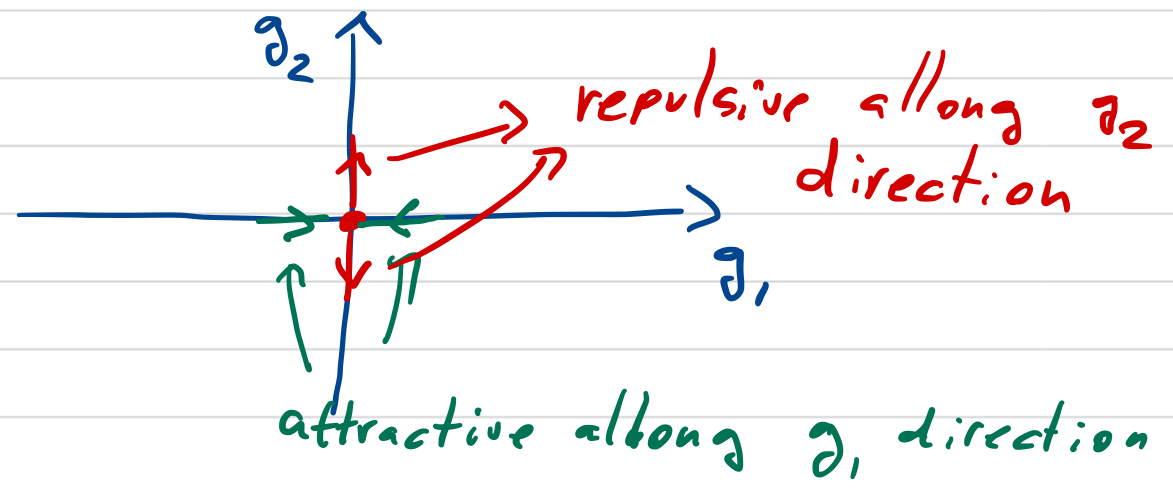
\includegraphics[width=0.7\linewidth]{gfx/RGtoy1}
	\caption{}
	\label{fig:rgtoy1}
\end{figure}
\item As for the other fixed point $g^*_1=\pm1$, $g^*_2=0$, we do an expansion of the form $g_i=g^*_i+\delta_i$ and linearize the $\beta$ function in $\delta_i$ for the respective component to get insight for the neighbourhood around the fixed point. We get
\begin{align}
	\frac{\md \vec{g}}{\md \ell} &= \frac{\md}{\md \ell} \begin{pmatrix}
		\delta_1 \\
		\delta_2 \\
	\end{pmatrix} = - \vec{\beta }|_{g_i=g^*_i+\delta_i} \nonumber\\
&= \begin{pmatrix}
 2 \delta_1 \\
 2\delta_2 \\
\end{pmatrix} + \mO(\delta_{1,2}) \nonumber \\
\Rightarrow \quad \delta_1(\ell) &= \delta_1(0) e^{2 \ell} \\
\delta_2(\ell) &= \delta_2(0) e^{2 \ell}.
\end{align} 
Therefore, the couplings are relevant (i.e. repulsive from the fixed point) for this fixed point, compare \ref{fig:rgtoy2}.

\begin{figure}[h!]
	\centering
	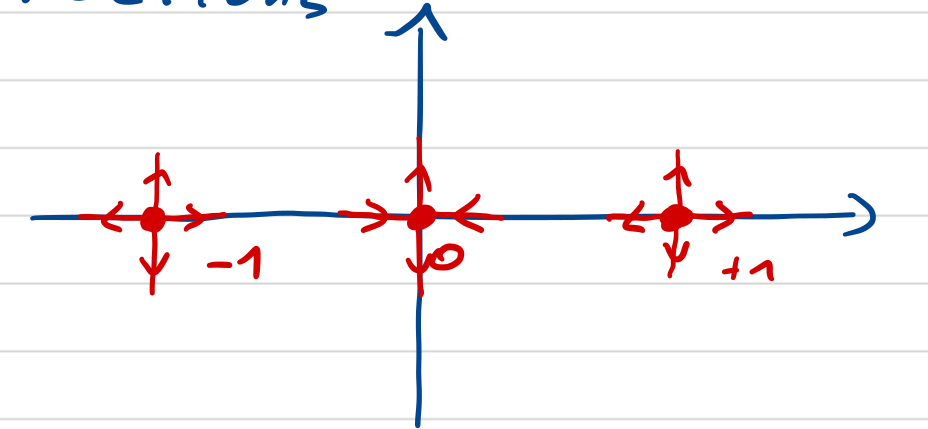
\includegraphics[width=0.35\linewidth]{gfx/RGtoy2}
	\; \longrightarrow \; 
	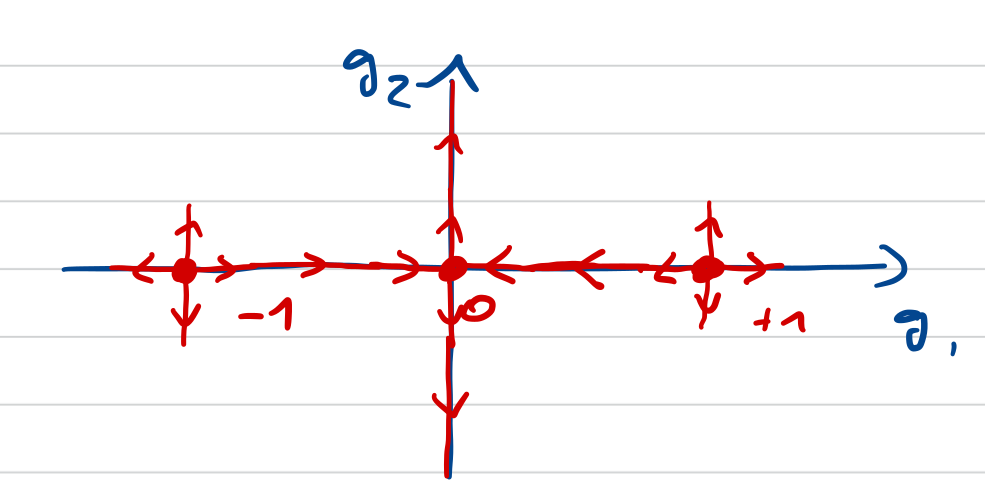
\includegraphics[width=0.35\linewidth]{gfx/RGtoy3}
	\caption{}
	\label{fig:rgtoy2}
\end{figure}
Note that we connected the flow lines in a way which is consistent with the properties of the above fixed points.\\
Now consider crossing the $g_1$-axis while $-1 < g_1 < 1$. If $g_2=0$, the RG flow will take us to the $g_1=g_2=0$ fixed point. At a fixed point the correlation length blows up and the system undergoes a phase transition.


 
\end{enumerate}

\subsection{TODO Anomalous dimension and dangerously (ir)relevant operators}
\begin{equation}
G_2(p) = \int \md^d x \bra{\Omega}\phi(x) \phi(y) \ket{\Omega} e^{ip(x-y)}\propto \left(\frac{1}{p^2}\right)^{1-\gamma_\phi(\lambda^*)}
\end{equation}
for $\lambda\rightarrow\lambda^*$ with $\beta(\lambda^*)=0$ is the scaling behaviour of the two-point correlator of a \emph{free massless scalar theory} of a field $\chi$ of mass dimension $[\chi]=1-\gamma_{\phi}(\lambda^*)$.
\subsection{TODO Two-point functions in real space and screening masses}
\begin{mybox}{}
	Screening mass
\begin{equation}
	\lim_{\abs{\vec{s}^2}\rightarrow\infty} G(s) \propto e^{- \abs{\vec{s}^2} m_{screen}}
\end{equation}
pole mass (i.e. gap mass) is temporal screening mass
\begin{equation}
	\lim_{\abs{{s}^0} \rightarrow\infty} G(s) \propto e^{- \abs{s^0}m_{pole}}
\end{equation}
and curvature mass
\begin{equation}
G^{(c)}(p) = \frac{1}{\Gamma^{(2)}}(p,-p).
\end{equation}
\end{mybox}
Scalar mass of Yukawa theory is screening mass in Yukawa potential between two charged fermions
\begin{equation}
	V(\vec{x})= - g^2 \int \frac{\md^3 q}{(2 \pi)^3} \frac{e^{i\vec{q}\cdot \vec{x}}}{\abs{\vec{q}}^2-m^2_\phi} = -\frac{g^2}{4\pi} \frac{1}{\abs{\vec{x}}} e^{-m_\phi \abs{\vec{x}}}
\end{equation}
which lead to the prediction of a scalar (the pion $\pi^0$) with a mass of $m_\phi \approx 200$ MeV mediating nuclear force.
\todo{think about this}




\subsubsection{An example of renormalization of quantum potential-- On the case of Euclidean massles $\phi^4$}
\begin{mybox}{}
	Euclidean $\phi^4$ quantum potential
	\begin{equation}
		\mathcal{V}(\phi)=\frac{m^2_0}{2} \phi^2 +\frac{\lambda_0}{4!} \phi^4 + \half \int \frac{\md^4 k}{(2 \pi)^4} \ln \left[\frac{m^2_0+\frac{\lambda}{2} \phi^2+k^2}{m^2_0+k^2}\right]
	\end{equation}
	such that the Euclidean massless $\phi^4$ quantum potential in counter term notation reads
	\begin{equation}
		\mathcal{V}(\phi) = \frac{\lambda}{4!}\phi^4 + \half \int \frac{\md^4 k}{(2 \pi)^4} \ln \left(1+\frac{\lambda \phi^2}{2 k^2}\right) +\frac{\delta_m}{2} \phi^2+\frac{\delta_\lambda}{4!}\phi^4.
	\end{equation}
	With the renormalization conditions
	\begin{align}
		\frac{\partial^2 \mV}{\partial \phi^2}|_{\phi=0} &\stackrel{!}{=} 0 \\
		\frac{\partial^4 \mV}{\partial \phi^4} |_{\phi=\mu} &\stackrel{!}{=} \lambda
	\end{align}
the renormalized potential reads
\begin{equation}
	\mV(\phi) = \frac{\lambda}{4!}\phi^4 + \frac{\lambda^2 \phi^4}{256 \pi^2}\left[\ln\left(\frac{\phi^2}{\mu^2}\right)-\frac{25}{6}\right]
\end{equation}
and has a minimum at
\begin{equation}
	\phi = \mu \exp\left[\frac{11}{6} - \frac{16}{3} \frac{\pi^2}{\lambda}\right]
\end{equation}
\end{mybox}
Derivation:
\begin{align*}
	\mV^{(2)}(0) &= \delta_m + \frac{\lambda \Lambda^2}{32 \pi^2} \stackrel{!}{=} 0 \\
	\mV^{(2)}(\mu) &= \lambda + \delta_{\lambda}+\frac{3\lambda^2}{32 \pi^2}\left[\ln \left(\frac{\lambda \mu^2}{2 \Lambda^2}\right)+\frac{11}{3}\right]\stackrel{!}{=}\lambda
\end{align*}



\subsection{The emergence of renormalizability}

\begin{mybox}{}
	Bare complex $\phi^4+\phi^6$ theory
	\begin{align}
	S[\phi] &= \int \md^d x \left[\partial_\mu \phi^\dagger \partial^\mu \phi + m^2_0(\Lambda) \phi^\dagger \phi \right.\\
	&\left.\frac{1}{4} \lambda^{(4)}_0(\Lambda) (\phi^\dagger \phi)^2 + \frac{1}{6} \lambda^{(6)}_0(\Lambda)(\phi^\dagger \phi)^3 \right] \nonumber.
	\end{align}
	The one-loop effective potential assuming constant $\phi^\dagger(x)\phi(x)$$:=\rho(x)=const.=:\rho$
	\begin{align}
	U(\rho) &= m^2_\Lambda \rho + \lambda_\Lambda \rho^2 + \Delta U^{(1)}(\rho) + \mO(\hbar^2)\\
	\Delta U(\rho) &= \half \int \frac{\md^d q}{(2\pi)^d} \ln(q^2+m^2_\Lambda+3\lambda_\Lambda \rho).
	\end{align}
	Then the derivatives of the one-loop effective potential are given by, using the notation $U(\rho)\equiv U^{(1)}(\rho)$,$m_\lambda\equiv m_0(\Lambda)$, $\lambda_\Lambda\equiv \lambda^{(4)}_0(\Lambda)$, $\gamma_\Lambda\equiv \lambda^{(6)}_0(\Lambda)$
	\begin{align}
	U^\prime(0) &= m^2_\Lambda + \frac{3}{2} \lambda_\Lambda \int \frac{\md^d q}{(2 \pi)^d} \frac{1}{q^2+m^2_\Lambda}\\
	U^{\prime \prime}(0) &= \lambda_\Lambda - \frac{9}{2} \lambda^2_\Lambda \int \frac{\md^d q}{(2 \pi)^d} \frac{1}{(q^2+m^2_\Lambda)^2}\\
	U^{\prime \prime \prime}(0) &= \gamma\Lambda + 27 \lambda^3_\Lambda \int \frac{\md^d q}{(2 \pi)^d} \frac{1}{(q^2+m^2_\Lambda)^3}
	\end{align}
	where we find a suppression of $\phi^6$ by quantum fluctuations
	\begin{equation}
	\frac{U^{\prime \prime \prime}(0)}{\lambda^{(6)}_0(\Lambda)} \propto \frac{\lambda^3_\Lambda \Lambda^2}{m^2_\Lambda}
	\end{equation}
	i.e. the contribution from the $\phi^6$ coupling in the action is completely dominated in the running of non-renormalizable couplings makes them irrelevant in the IR.
\end{mybox}
We have seen other ways to understand this emergence of renormalizability: the beta function formalism for non-renormalizable coupling and the Wilsonian flow of non-renormalizable couplings.




\subsection{Concepts from critical phenomena theory - a prelude to the Wilsonian RG flow approach}
\subsubsection{Correlation length or mass gap}
One of the most important aspects of critical phenomena theory, as well as in QFT in general, is to determine the mass gap, or equivalently the correlation length, and in particular its dependence on the couplings. What does this mean ?
\\
\begin{mybox}{Correlation length}
	The correlation length $\xi \in \mR_{\geq 0}$ is roughly the minimal length at which macroscopic properties of a theory remain valid.
\end{mybox}
In other words, if somebody gave us a piece of material whose linear dimensions are all larger than the correlation length, we would find that piece of material will behave pretty much the same as any other piece of the same material, as long as the size of the material is larger than its correlation length.
\begin{mybox}{Mass gap}
The mass gap is just the inverse correlation length $m = 1/\xi$.
\end{mybox}
The name stems from QFT:\\
If the system is gapped, the temporal correlation function will decay exponentially with the Euclidean time separation, i.e.
\be 
\langle \phi(\vec{x},t) \phi(\vec{x},t^\prime)\rangle \approx e^{-\abs{t-t^\prime} m}.
\ee 
Therefore, gapped here means in the sense of having finite correlations talking in terms of correlation length. Subsystem making up a system would appear as if they were closed and therefore disjointly combined into the system, where the size of the subsystem is defined by the correlation length. If $\xi\rightarrow 0$, then $m\rightarrow \infty$ which means that the two-point correlator vanishes. With a vanishing correlation length, you would basically never create particles in the theory because there are no interactions, every correlator vanishes. This is because all the $n$-point correlators are made up of $2$-point correlators for quadratic actions.\\
However, in relativistic field theory this implies that any space-time correlator has to have the same exponential dependence
\be 
\langle \phi(x^\prime) \phi(x) \rangle \approx e^{- \abs{x-x^\prime} m} \quad x,x^\prime \in \mR^{1,3}.
\ee 
As we will see later, this implies that with every RG-transformation, i.e. with every iteration, you go to smaller and smaller correlation lengths $\xi^\prime < \xi$. We look at subsystems with less and less information with every iteration, as they correlate in a smaller radius $\xi^\prime,\xi^{\prime \prime}$. This also means that every \todo{is that true ?} has a defined correlation length. I guess that the extreme case of $\xi=\infty$ is just not solvable as you basically account for every interaction which is possible, while $\xi=0$ is boring as nothing happens.	



















\section{On the Wilsonian renormalization idea -- Wilsonian effective field theory}
\subsection{Conceptual idea}
The original understanding of renormalization was:
\begin{enumerate}
	\item The cutoff $\Lambda$ is merely a way to regulate divergent integrals without any physical meaning.
	\item Renormalization is a trick to remove the cutoff-dependence in physical amplitudes. This procedure allows us to take $\Lambda \rightarrow \infty$ without encountering any divergences.
	\item This comes at the cost of losing predictability for a number of physical masses and coupling.
	\item In a renormalizable theory, only a finite number of such physical couplings must be taken as input parameters from expereiment to end up with a well-defined (otherwise predictive) theory.
\end{enumerate}
The Wilsonian approach gives a different interpretation:\\
We should think of QFT as an \emph{effective description} accurate only for energies below an intrinsic cutoff $\Lambda_0$. At energies beyond $\Lambda_0$ the field theory picture does not correctly model the microscopic degrees of freedom.\\
For example, QFT neglects gravity but all matter gravitates and the effects of gravity become non-negligible (compared to other forces) near the Planck scale
\begin{equation}
	\Lambda_0 \propto M_{pl} = \frac{1}{\sqrt{8  \pi G_N}} \approx 10^{18} \mathrm{GeV}.
\end{equation}
The only know theory that is UV finite and asymptotes to a weakly coupled QFT in the infrared is string theory, which abandons the concept of pointlike particles, replacing them with excitations of a one-dimensional string of length $l_s$. The string length is the intrinsic cutoff of the low-energy effective QFT. At distances near $l_s$, the theory deviates from a regular field theory in that it becomes non-local, thus avoiding UV divergences and arbitrary input parameters.\\
\\
Integrating out the degrees of freedom between the regulator $\Lambda$ and an even small cutoff $\Lambda_0 < \Lambda$ (thus avoiding large log corrections for $\Lambda_0 \ll \Lambda$) yields the Wilsonian effective action $S^{eff}_W$ (which only accounts for the remaining degrees of freedom below $\Lambda_0$).\\
When computing correlators at scales below $\Lambda_0$ via $S^{eff}_W$, only momenta $\abs{k} \leq \Lambda_0$ appear in the loops since all effects of the modes with $\Lambda_0 < \abs{k} < \Lambda$ are already encoded in $S^{eff}_W$. This \emph{Wilsonian effective action} is \emph{not} to be confused with the quantum effective action $\Gamma[\varphi]$, which gives the full quantum theory ($=$ includes all quantum effects) already at tree-level (no loops!).\\
$S^{eff}_W$ includes only those quantum effects due to the integrated-out modes $k$ between $\Lambda_0 < \abs{k} < \Lambda$ and loops must still be performed.
\begin{enumerate}
	\item The successive application of integrating out the degrees of freedom with $\Lambda_0 < \abs{k} < \Lambda$ gives rise to the renormalization (semi)-group (semi because we can only lower the cutoff; there does not exist an inverse operation).
	\item The running couplings in the Wilsonian picture are interpreted as the dependency of the couplings in $S^{eff}_W$ on the cutoff. This identifies $\Lambda_0$ as the renormalization scale $\mu$. \\
	$\Rightarrow$ The effective couplings $\lambda(\Gamma_0)$ are defined by specifying observables computed from the effective action cutoff $\Lambda_0$.\\
	This replaces our previous renormalization condition fixing $\lambda(\mu)$.
	\item $\Rightarrow$ Even with renormalization our theory remains an effective theory to the extent that all couplings are really input parameters and cannot be computed from first principles without knowing the underlying theory.
\end{enumerate}
\subsubsection{Motivation from statistical physics}
\begin{mybox}{Correspondence}
	One can interpret a $\md$- spatial dimensional thermal partition function of a QFT as a $(\md+1)$-dimensional system in classical statistical mechanics.
\end{mybox}
This connection is striking, given how different the quantum realm is from the classical one. Somehow all of the non-triviality of the quantum world is packed into an extra classical dimension. However, you should note that there are quantum systems which cannot be written as a statistical mechanics system, i.e. their probability wieght in the path integral is not positive. These systems are very poorly studied numerically, precisely because a statistical interpretation is not possible and simulations become prohibitively costly.









\subsection{Floating UV cutoff and Wilsonian effective action}
\begin{mybox}{}
	The generating function with explicit cut-off reads
	\begin{equation}
	Z[0] = \lim_{\Lambda_0 \rightarrow \infty} \int [\mD \phi_0]_{\Lambda_0} e^{i S[\phi_0]} \text{ with } [\mD \phi_0]_{\Lambda_0} := \prod_{\abs{k}<\Lambda_0} \md \phi_0 (k).
		\end{equation}
	The Wilsonian effective action $S_\Lambda$ is the effective action at scale $\Lambda:=b\Lambda_0$
	\begin{equation}
	\label{eq:wilsonianeffectiveaction}
		\int [\mD \phi_0]_{\Lambda_0} e^{i S[\phi_0]} =: \int [\mD\phi]_{b\Lambda_0} e^{iS_\Lambda[\phi]} \text{ with } 0<b=\frac{\Lambda}{\Lambda_0}<1.
	\end{equation}
	"Integrating out" of high momentum modes by separation of modes
	\begin{align}
		\phi_0(k) &= \phi(k) +\hat{ \phi}(k)\label{eq:wilsonianSplittingmodes} \\
		\text{with } \phi(k) &= 0 \text{ for } b\Lambda_0<k<\Lambda_0 \quad (\text{low mode})\\
		\hat{ \phi}(k) &= 0 \text{ for } 0<k<b\Lambda_0 \quad (\text{ high mode})
	\end{align}
allows us to split the path integral and pull the partof the action that only depends on the low modes $\phi$ out of the high mode path integral $\int \mD \hat{ \phi}$
	\begin{align}
		\int [\mD \phi_0]_{\Lambda_0} e^{i S[\phi_0]} \stackrel{\ref{eq:wilsonianSplittingmodes}}{=}& \int [\mD\phi]_{b\Lambda_0}\left[e^{iS[\phi] \int [\mD \hat{ \phi}]} e^{i \hat{S}[\phi,\hat{ \phi}]}\right]  \\
		\text{ with } \hat{S}[\phi,\hat{ \phi}] =& S[\phi+\hat{ \phi}]-S[\phi]
	\end{align}
where mixed terms in $\phi,\hat{ \phi}$ arise in $S[\phi+\hat{ \phi}]$.\\
Executing the high mode path integral
\begin{align}
	\label{eq:reference4}
&	\int [\mD \hat{ \phi}] e^{i \hat{S}[\phi,\hat{ \phi}]} =: e^{i S^\prime[\phi]}\\
&S_\Lambda[\phi] = S[\phi] + S^\prime[\phi] = S[\phi] -i \ln \int [\mD \hat{ \phi}] e^{i (S[\phi+\hat{ \phi} ] - S[\phi])}
\end{align}
is the essential step of the construction of $S_\Lambda$. The integration \ref{eq:reference4} gives rise to all possible interaction terms that are allowed by the symmetries of the original action. This includes non-local interactions at the scale of $\Delta x \propto \frac{1}{\Lambda}$ and non-renormalizable terms.
	
\end{mybox}
\subsection{Wilsonian RG flow on the example of scalar theory}
Let us reiterate the idea of Wilsonian renormalization. Wilson' s idea of RG flow is to always put a cutoff in your theory. This is quite natural from the point of view of effective field theories. All QFTs employed today are emergent QFTs and not genuine ones (i.e. QCD need String theory as UV completion). Of course, how exactly one regulates the theory is not unique, and in fact it can often break symmetries (hard cut-off breaks gauge invariance because gauge symmetry transformation can be seen as reshuffling of the momentum modes, while a lattice cut-off breaks rotational and translational symmetries).\\
The next step of the RG flow is to integrate out short distance features of the theory and keep long distance ones.
This can often be done in several ways. By doing this, we will generate a theory which no longer has short-distance components of the fields (i.e. high momentum Fourier modes), so the resulting thoery will not be good for asking questions which depend heavily on short-distance modes. However, we are most often interested in the opposite limit, which is the low-energy limit of the theory. This tells us what particles we see, and how the system behaves macroscopically. However, this step will generate infinitely many terms in the low-energy theory. These terms are "non-renormalizable" from the point of view of the counter-term approach (they require infinitely many counterterms to deal with). Bet these terms will be harmless in the infrared as they will be \emph{irrelevant} for observations at long distances.\\
\\
Consider now the usual $\phi^4$ theory. We consider two cut-offs for the theory, $\Lambda$ and $\Lambda^\prime$, where $\Lambda^\prime >\Lambda$. We want to integrate momentum modes in the shell $\Lambda-\Lambda^\prime \equiv \Delta \Lambda$ in the limit of an infinitesimally small momentum-shell, i.e  $\Delta \Lambda \rightarrow 0$. What is the idea here ?\\
Exactly following Wilson's approach, we integrate a small amount of momentum modes from the energy space $\Delta$ whilst retaining the cut-off $\Lambda$ in the  theory, that is the result will depend on the cut-off. We however integrate out any dependence above our cut-off. This first iteration, i.e. the integration of $\Delta\Lambda$, will yield a shift in the parameters of this theory, i.e. $\lambda$ and $m$. We can then continue with further iterations, integration out $\Lambda-\Lambda^{\prime \prime }$ and so forth. Every iteration will yield a subsequent step in the shift of the parameters of our theory. The shifts for relevant operators are, as the name suggests, interesting and the point towards constructive points in the flow trajectory. This sounds nebulous and will be cleared up in the following, but essentially the iterations give the individual steps of a flow trajectory of this parameter.\\
As for the first iteration step of this theory, we start of by making the ansatz $\phi=\phi^\prime +\tilde{\phi}$ where
\bse 
\phi^\prime = \int_{k^2 \leq \Lambda^2} \int \frac{\md^D k}{(2 \pi)^D} e^{ikx} \phi^\prime(k),\; \tilde{\phi} = \int_{\Lambda^2 < q^2 \leq {\Lambda^\prime}^2} \frac{\md^D q}{(2 \pi)^D} \tilde{\phi}(q) e^{iqxx}.
\ese 
Our goal is to integrate out $\tilde{\phi}$, i.e. all the modes of the field above out cut-off. We consider a thin momentum-shell, which makes the calculation easier as we can do everything to $\mO({\Delta \Lambda}^2)$ and replace
\bse 
\int \frac{\md^D q}{(2\pi)^D} \frac{1}{q^n} = \int \md \Omega(S^{D-1}) \int_{\Lambda}^{\Lambda^\prime} \frac{\md q}{(2 \pi)^D} q^{D-n-1} \approx \Omega(S^{D-1}) \Lambda^{D-n-1} \frac{\Delta \Lambda}{(2\pi)^D}.
\ese 
This yields the first iteration shift
\begin{align}
	\label{eq:renormWilson1flow}
\frac{m^2}{2 } &\rightarrow \frac{{m^\prime}^2}{2} = \frac{m^2}{2} + \Lambda^{D-3} \Delta \Lambda \frac{\Omega(S^{D-1}) 3 \lambda}{2 (2\pi)^D}\\
\lambda &\rightarrow \lambda^\prime = \lambda - 9 \lambda^2 \frac{\Lambda^{D-5} \Delta \Lambda}{(2 \pi)^D} \Omega(S^{D-1})\nonumber
\end{align}
to first order in $\Delta \Lambda$. We have successfully performed an RG flow iteration and obtained new couplings $m^\prime,\lambda^\prime$. However we have also generated an infinite tower of couplings, any coupling in
fact which is allowed by the symmetries $\phi \rightarrow - \phi $ the space-time symmetries.\\
\subsubsection{Dimensionful couplings on the example of $\phi^4$}

Consider the dimensionful coupling $m$ for free $\phi^4$. Of course, the theory here is free, so everything is computable, and we know that physically we have that the mass-gap is given by the bare mass of the theory, because we can compute the two-point correlator and get that they decay as $\propto e^{-m \abs{x-y}}$, where $m$ is the bare mass, which now will not get renormalized if measured in terms of some physical, fixed scale. However, in the context of RG flow dimensionful quantities such as mass are to be expressed in units of the cutoff scale. Furthermore since the cutoff scale changes under the RG flow, the mass will change under the RG flow, not because of integration effect of the short distance momenta,  but because we have changed the unit of measurement. In other words, we take that the dimensionless mass parameter $g$ at scale $\Lambda$ is given by
\be
g_m(\Lambda) = \frac{m^2(\Lambda)}{\Lambda^2}.
\ee 
Now it is easy to see how $g(\Lambda)$ changes as we shift the cutoff to $\Lambda^\prime$
\begin{align*}
	g_m(\Lambda^\prime) &= g_m(\Lambda) \frac{\Lambda^2}{(\Lambda^\prime)^2} = g_m(\Lambda) \left(\frac{\Lambda^\prime + \Delta \Lambda}{\Lambda^\prime}\right)^2 \\
	&\approx g_m(\Lambda) + 2 \frac{\Delta \Lambda }{\Lambda^\prime} g_m(\Lambda) + \mO\left(\frac{\Delta \Lambda}{\Lambda}\right).
\end{align*}
How does $g(\Lambda)$ change for infinitesimal $\Delta \Lambda$ ?
\bse 
\Lambda^\prime \frac{g_m(\Lambda^\prime) - g_m(\Lambda) }{\Lambda^\prime -\Lambda } \approx  -2 g_m(\Lambda).
\ese 
For $\Lambda^\prime \rightarrow \Lambda$
\be 
\label{eq:renormWilsonmass}
\Lambda \frac{\md g_m(\Lambda)}{\md \Lambda} = - 2 g_m(\Lambda).
\ee 
This is the RG flow equation for the mass parameter $g_m$ in the free scalar theory, as the cutoff is varied. This equation is nothing but a reflection of the fact that $m^2=g(\Lambda) \Lambda^2$ is RG invariant. Starting from this fact, we can also derive the RG flow equation
\begin{align*}
	0 \stackrel{!}{=}& \frac{\md}{\md \Lambda} m^2=g_m^\prime(\Lambda) \Lambda^2 +2 \Lambda g_m(\Lambda) \\
	\Leftrightarrow \quad \Lambda \frac{\md g_m(\Lambda)}{\md \Lambda } =& - 2 g_m(\Lambda).
\end{align*}
Considering the coupling parameter on the other hand, we have $[\lambda]= 4-D$, therefore we define $g_\lambda = \frac{\lambda}{\Lambda^{4-D}}$ to be dimensionless. Consider the pure scaling, i.e. without quantum corrections. We know then that $\lambda$ is supposed not to run under the scaling. This means, since $\lambda(\Lambda) = g_\lambda \Lambda^{4-D}$ that
\begin{align}
	\label{eq:renormWilsoncoupling}
	0 & \stackrel{!}{=} \Lambda \frac{\md}{\md \Lambda } \lambda(\Lambda)\nonumber \\
	&= \left[\Lambda \partial_\Lambda g_\lambda(\Lambda) + (4-D) g_\lambda(\Lambda) \right] \Lambda^{4-D} \nonumber \\
	\Leftrightarrow \quad \Lambda \frac{\md g_\lambda}{\md \Lambda} &= - (4-D) g_\lambda (\Lambda) 
\end{align}
which is the RG flow equation for the coupling.


\subsubsection{$D=4$ and the one-loop beta function for $\lambda$ and $m^2$}
Rewriting the flow equations \ref{eq:renormWilson1flow} in terms of the mass and coupling parameter with respect to the new cut-off yields
\begin{align*}
	\Lambda \frac{\md g_m(\Lambda)}{\md \Lambda }&= -2 g_m(\Lambda) -3 \lambda(\Lambda) \frac{\Omega(S^3)}{(2 \pi)^4}\\
	\Lambda \frac{\md \lambda(\Lambda)}{\md \Lambda} &=9 \lambda^2 \frac{\Omega(S^3)}{(2 \pi)^4},
\end{align*}
where the first term for $g_m$ is just the classical flow term as seen in \ref{eq:renormWilsonmass} whilst the second term for $g_m$ comes from the one-loop renormalization of the mass. The coupling term only contains the one-loop correction, as the classical RG flow \ref{eq:renormWilsoncoupling} vanishes in $D=4$.
\\
These equation can be rewritten using the parametrization $\Lambda = e^{-\ell} \Lambda_0$, where $\Lambda_0$ is some reference scale\footnote{Could for example be the scale at which our theory is defined. We called this scale $\Lambda$ throughout the previous sections, and $\Lambda^\prime$ the scale to which the theory flows. But in the lst step of deriving the flow equations, we changed the running scale to $\Lambda$. Unfortunately, this means that we need a new name for the UV scale we started with, and $\Lambda_0$ was chosen to be this new name.} so that when $\ell=0$ we have not flowed at all. Then the flow equations flow according to
\begin{align}
	\frac{\md g_m}{\md \ell} &=2 g_m (\Lambda) +3 \lambda(\Lambda) \frac{\Omega(S^3)}{(2 \pi)^4},\\
	\frac{\md \lambda}{\md \ell} &= - 9 \lambda^2 \frac{\Omega(S^3)}{(2 \pi)^4}.
\end{align}


\subsubsection{The $\beta$-functions in $D=4-\epsilon$ dimensions and the Wilson-Fischer fixed point}
Considering the flow equations for $D=4-\epsilon$ dimensions with resummed interactions one has
\begin{align}
	\frac{\md g_m}{\md \ell} &= 2 g_m + \frac{3g_\lambda}{1+g_m} \frac{\Omega(S^{D-1})}{(2 \pi)^D},\\
	\frac{\md g_\lambda}{\md \ell} &= (4-D) g_\lambda - \frac{9 g^2_\lambda}{(1+g_m)^2} \frac{\Omega(S^{D-1})}{(2 \pi)^D}.
\end{align}
Now let us try to find the fixed point of these equations for small $\epsilon =4-D$, i.e. a point when the RHS of both equations vanishes. Firstly, there is a trivial fixed point when $g_\lambda =g_m=0$. This corresponds to the theory being massless and free.\\
Another fixed point, the Wilson-Fisher fixed point, can be found as follows. Set the RHS of the second equation above to zero. Then we have a solution
\be 
g^*_\lambda = \frac{\epsilon (2 \pi)^D (1+g^*_m)^2 }{9 \Omega(S^{D-1})}.
\ee 
Now ew must find $g^*_m$ such that the first equation also vanishes. We have that
\bse 
g^*_m = -\frac{3 g^*_\lambda \Omega(S^{D-1})}{2(1+g^*_m) (2 \pi)^D} = - \frac{\epsilon}{6} + \underbrace{\mO(g^*_m)}_{\mO(\epsilon^2)}.
\ese
Now let us expand $g_\lambda = g^*_\lambda+\tilde{g}_\lambda$ and $g_m = g^*_m + \tilde{g}_m$. We have that
\begin{align*}
\frac{\md \tilde{g}_m}{\md \ell} &= \frac{\md g_m}{\md \ell } = 2 g_m + \frac{3g_\lambda}{1+g_m} \frac{\Omega(S^{D-1})}{(2 \pi)^D} \\
&\approx \left(2-\frac{\epsilon}{3}\right) \tilde{g}_m + \tilde{g}_\lambda 3 \frac{\Omega(S^{D-1})}{(2 \pi)^D},\\
\frac{\md \tilde{g}_\lambda}{\md \ell} &= \frac{\md g_\lambda}{\md \ell} = \epsilon g_\lambda - \frac{9 g^2_\lambda}{(1+g_m)^2} \frac{\Omega(S^{D-1})}{(2 \pi)^D}\\
&\approx -\epsilon \tilde{g}_\lambda,
\end{align*}
where we only kept terms of leading order in $\epsilon$ and $\tilde{g}_i$. Note that the beta functions are then found by looking at
$\beta_i(\ell) = - \frac{\md g_i}{\md \ell}$.\\
The flow equations can therefore be written as
\be 
\frac{\md \vec{\tilde{g}}}{\md \ell } = \frac{\md}{\md \ell} \begin{pmatrix}
	\tilde{g}_m \\
	\tilde{g}_\lambda \\
\end{pmatrix}
= \begin{pmatrix}
	2-\frac{\epsilon}{3} & 3 \frac{\Omega(S^{D-1})}{(2 \pi)^D}\\
	0 & -\epsilon \\ 
\end{pmatrix}
\vec{\tilde{g}}
\equiv 
T \vec{\tilde{g}}.
\ee 
The eigenvalues of $T$ are easily found by considering the characteristic polynomial $\det(T-y\mI)=0$, one has
\bse 
y_1 = 2 -\frac{\epsilon}{3}, \quad y_2 = -\epsilon.
\ese 
Now let us call $\vec{\phi}_1$ and $\vec{\phi}_2$ the two right eigenvectors\footnote{Since $T$ is not symmetric, the left and right eigenvectors need not be the same.} Because the eigenvalues are distinct, these eigenvectors must form a basis. Writing $\vec{\tilde{g}}$ in terms of $\vec{\phi}_1$ and $\vec{\phi}_2$ we have
\be 
\tilde{g} = u_1 \vec{\phi}_1 + u_2 \vec{\phi}_2,
\ee 
so that the flow equation becomes
\be 
\frac{\md u_i}{\md \ell} = y_i u_i \; \Rightarrow \; u_i(\ell) = e^{y_i \ell} u_i(0).
\ee 
Notice that $u_1$ increases in magnitude while $u_2$ decreases.\\
We now want to consider how might the correlation length of this system behave as we vary the $u_1(0)$ and $u_2(0)$, which are some bare couplings of our system.\footnote{In actual experiments, one typically has no control over $u$-variables, but has control more likely over some bare couplings of the Lagrangian or Hamiltonian. Just a toy model here, so ignore the issue.}
Notice that when we were considering the couplings $g_m$ and $g_\lambda$, both were relevant around the point $g_m=g_\lambda=0$. However, around the new fixed point $g^*_m, g^*_\lambda$ this is no longer the case. Only one combination of them is relevant.\\
Let us analyse this situation a bit further. Note that the correlation length must scale in our system with $\ell$. Recall that the correlation length $\xi$ is defined as a correlation length in units of the cutoff. The cutoff is given by $\Lambda = e^{-\ell} \Lambda_0$, so $\xi(\ell)/\Lambda$ must be RG invariant, because it represents a measurable physical quantity which does not depend on which modes we keep in our Lagrangian. Therefore, we must have that
\be 
\xi(\ell) = e^{-\ell} \xi(0).
\ee 
On the other hand, $\xi(\ell)$ can depend on $\ell$ only through $u_1$ and $u_2$ (and all the other couplings of $\phi^4$ which we ignored here, they turn out to be irrelevant). But the dependence on $u_1$ and $u_2$ is no arbitrary. Namely, we first note that in order to scale properly we must have that $\xi \propto \frac{1}{(u_1)^{1/y_1} }$ or $\xi \propto \frac{1}{(u_2)^{1/y_2}}$, times a function of $u_1, u_2$ which is invariant under the RG flow. Such a function must be a function of the ratio $\frac{(u_2)^{1/y_2} }{(u_1)^{1/y_1}}$, which is RG invariant. So we must have
\be
\xi = \frac{1}{(u_1)^{\frac{1}{y_1} }} f\left( \frac{(u_2)^{1/y_2} }{(u_1)^{1/y_1} }\right)
\ee 
where $f$ is a universal function, up to perhaps an overall constant.\\
The variables $u_1$ and $u_2$ are sometimes referred to as \emph{scaling variables}. Note that the scaling variables are just a combination of our couplings, so they can be though of as a different basis of couplings. The advantage of using $u_i$ is that their RG flow is simple, they evolve exponentially with $\ell$ which parametrizes the RG flow.



\subsection{RG flow and scaling variables}
After this example of a RG flow analysis, we will start to discuss the concepts in a more abstract fashion now.\\
To begin with imagine that all the dimensionless couplings (i.e. couplings expressed in terms of the dimension of the cutoff) of the system are organized into a vector $\mathbf{g}=(g_1,g_2,\dots)$. We then integrate over UV degrees of freedom, so that our regulator $\Lambda$ becomes $\Lambda^\prime = e^{-l} \Lambda$. The vector $\mathbf{G}$ then changes into $\mathbf{g}^\prime(\mathbf{g})$, which is a function of $\mathbf{g}$ only. Since we take $\ell$ to be continuous\footnote{This is possible in the QFT context, but in stat. mech. the RG iteration may have to be a discrete process, like we have seen in the case of $1d$ Ising model.}, to leading order in $\ll$ we must  have
\be 
\label{eq:renormWilsonFlow}
\mathbf{g}^\prime = \mathbf{g} - \ell \mathbf{\beta}(\mathg) + \mO(\ell),
\ee 
where $\mathbf{\beta}$ are the expansion coefficients. The sign is conventional. Viewing $\mathg^\prime$ as a function of $\ell$ and $\mathg$ above as the value of $\mathg(\ell)|_{\ell=0}$, we have that the above equation in the limit $\ell \rightarrow 0$ becomes
\be 
\frac{\md \mathg}{\md \ell } =-\vec{\beta}(\mathg).
\ee
This is the RG flow equation. Notice that we in reality have infinitely many couplings $g_i$. However, typically there is only a few relevant couplings, so that the IR physics depends most strongly on only a few parameters. It is this feature that is responsible for the universality across many different systems.\\
In general, the exact beta functions are not calculable. Instead, we want to analyse the equations \ref{eq:renormWilsonFlow} in the vicinity of a fixed point. A fixed point of the IR equations is a point $\mathg^*$ such that $\beta(\mathg^*)=$. Then the RG equations indicate that all the dimensionless couplings $\mathg=\mathg^*$ remain constant along the RG flow.\\
If we expand the $\beta$-functions $\vec{\beta}(\mathg)$ around $\mathg^*$ we have
\be 
\mathbf{\beta}( \mathg^* + \tilde{\mathg}) = T \tilde{\mathg} +\mO(\tilde{g}),
\ee 
where $T$ is a matrix acting on the components of the vector $\tilde{\mathg}$. Solving\footnote{The equation above is only tenable if the number of couplings is finite. However, this is not the case. In practice, one would truncate the space as most couplings in the space are irrelevant and will not have a strong effect on the IR physics.} for the eigenvalues of $T$ yields the eigenvalues $y_1,y_2,\dots$. We will order these eigenvalues so that $y_1>y_2>y_3>\dots$ Note that generically we have no reason to expect that the eigenvalues $y_i$ are degenerate, unless a symmetry transformation relates some of the couplings $\mathg$. However then one does not need to consider separate couplings, and one may just as well put all of the couplings related by a symmetry to zero, save one. Generically, we would therefore expect that all the eigenvalues are distinct.\\
If this is the case, one can show that the right eigenvectors $\phi^i$ associated to these eigenvalues are linearly independent, so that we can write $\tilde{\mathg}= \sum_i u_i \phi^i$. Therefore. the scaling variables $u_i$ are defined near the fixed point to be some linear combination of $g_i$ couplings, where $g_i$ are deviations from the fixed point. The couplings $g_i$ couple linearly to some operators in the action.Plug this into the RG equation, the $u_i$ then obey the following flow equation
\be 
\frac{\md u_i}{\md \ell} = y_i u_i \; \Rightarrow \; u_i(\ell) = e^{y_i \ell} u_i(0).
\ee 
\begin{mybox}{Classification of scaling variables}
Now we come to the classification of the scaling variables $u_i$. We say that the scaling variable $u_i$ is
\begin{enumerate}
	\item \emph{Relevant} if $y_i >0$,
	\item \emph{Irrelevant} if $y_i <0$,
	\item \emph{Marginal} if $y_i=0$.
\end{enumerate}
The terms are chosen to reflect the couplings $u_i$ in the IR. Note that the marginal scaling variables do not transform under the RG flow, but this need not be true if we keep terms of higher order in $\tilde{g}$. In fact, generically all the couplings will flow, but it may happen that to first order in $\tilde{g}$ some couplings do not transform. Then we usually say that the coupling is marginally relevant or irrelevant depending on whether it grows or decays as $\ell$ grows.
\end{mybox}
There is a subtlety here which we have to address before moving on.
\subsubsection{Subtlety on irrelevant operators} 
It is not quite true when we say that irrelevant operators can simply be dropped. A more precise statement is that they do not (under certain assumptions) influence the IR physics. However, the dimensionless couplings $g_i$ which are irrelevant do not necessarily go to zero. Rather the statement is that whatever their starting point is at $\Lambda_0$, the RG flow curves will pass very close to each other. 

\begin{figure}[h!]
	\centering
	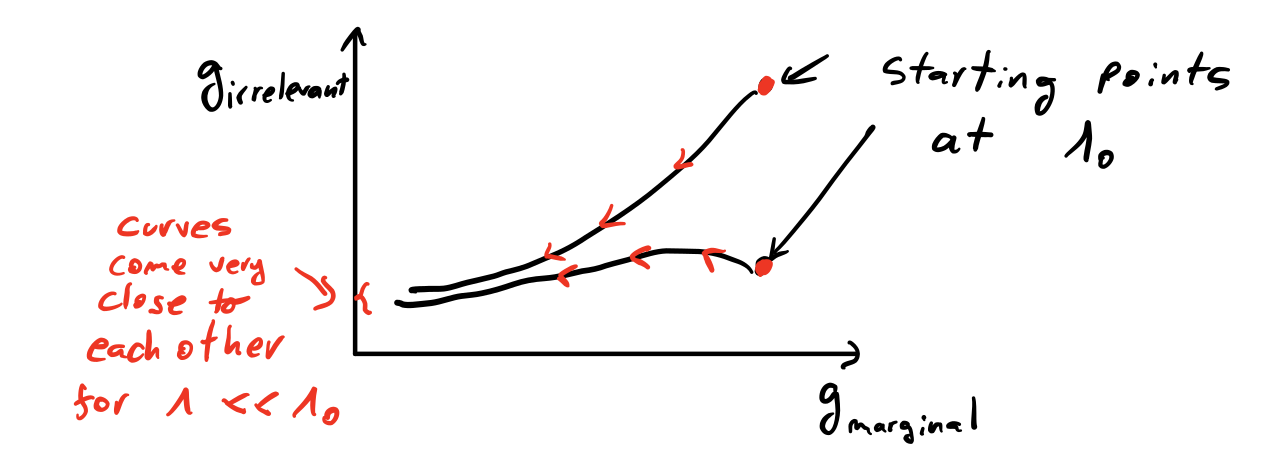
\includegraphics[width=0.7\linewidth]{gfx/RG1}
	\caption{}
	\label{fig:rg1}
\end{figure}

The marginally irrelevant couplings will also attract in the IR, but the effect will be logarithmic in the ratio 
of the UV and IR scales, so its effects can be felt to very deep IR. Considering a plot with a relevant coupling, we have

\begin{figure}[h!]
	\centering
	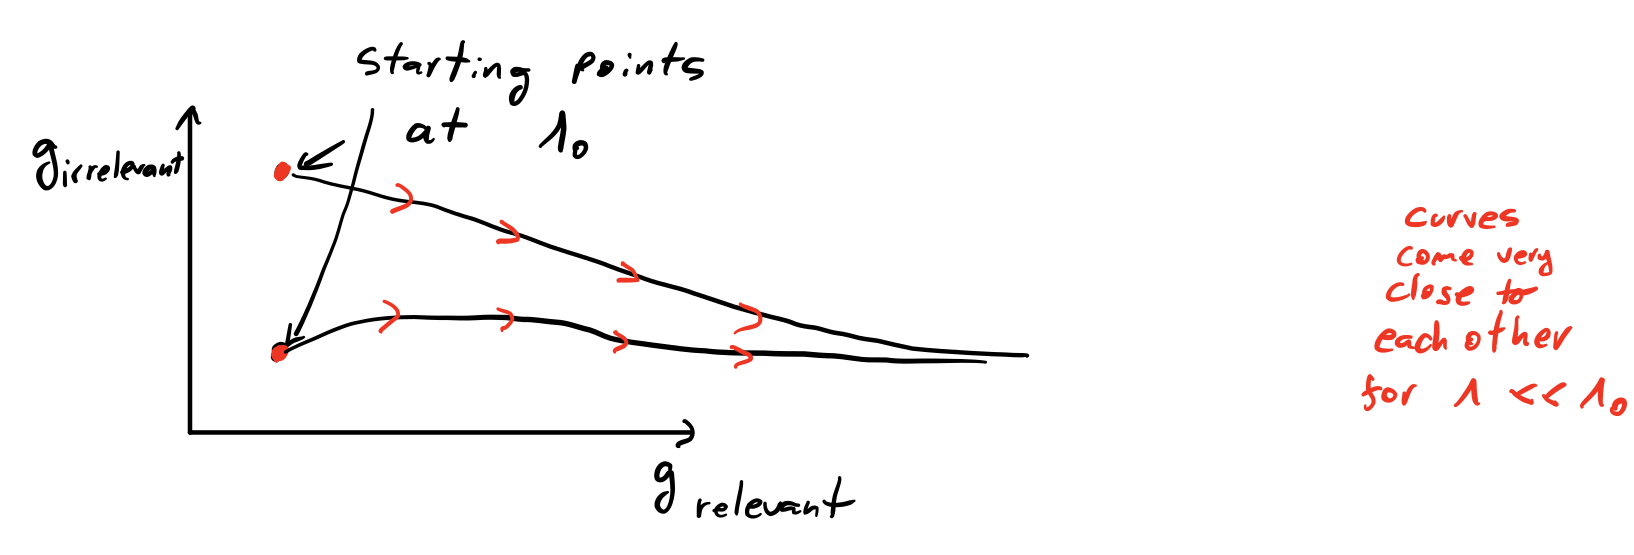
\includegraphics[width=0.7\linewidth]{gfx/RG2}
	\caption{}
	\label{fig:rg2}
\end{figure}

Note that these results involve some assumptions.
\begin{enumerate}
	\item The labels "relevant" and "irrelevant" must be in relation to some fixed point, and we usually mean a Gaussian fixed point. 
	\item The argument which was given by Polchinski in $1984$ involves an assumption that all the coupling are small in the range that we analyse the flow. This means that, as we flow to the IR, the irrelevant couplings move along different flows, and come close together before the perturbation theory breaks down.
\end{enumerate}
Under these assumptions we are allowed to change the UV scale $\Lambda \rightarrow \Lambda^\prime$ keeping only the relevant couplings without disturbing the physics at low energies.



\subsubsection{Continue with recipe for analysis}
Note that RG flow can alternatively be interpreted as acting on the scaling operators, instead of the scale and the couplings.













Now consider an observable $\mO$ that has a dimension of $[\mO]=\Delta$, measured in units of the cutoff $\Lambda$. Then we know that $\mO/\Lambda^\Delta$ must be an invariance of the RG flow. However, we also know that $\Lambda \rightarrow e^{-\ell} \Lambda_0$, so that $\mO$ must scale as
\be 
\mO(\ell) = e^{-\Delta \ell} \mO(0).
\ee 
However, the operator $\mO$ depends on the $\ell$ only implicitly through the couplings $u_i$, i.e. $mO(u_1,u_2,\dots)$. The observable $\mO$ must therefore have a dependence on $u_i$ such that it reproduces the above scaling. Since $1/(u_1)^{\Delta/y_1}$ scales as $\mO$ we get
\be 
\label{eq:renormWilsonScalingLaws}
\mO = \frac{1}{u_1^{\frac{\Delta}{y_1} } } f\left(\frac{(u_2)^{\frac{1}{y_2}} }{(u_1)^{\frac{1}{y_1} } }, \frac{(u_3)^{\frac{1}{y_3} } }{(u_1)^{\frac{1}{y_1}}} ,\dots \right).
\ee 
These are the famous scaling laws, which were discovered in specific systems before the advent of RG. Note that the above combinations have branch-cuts if $y_i<0$. Bu we may always choose the scaling variables so that they are positive by changing the sign in the expansion of $\tilde{\mathg}$.\\
Let us take $\mO$ to be the correlation length $\xi$, so that $\Delta=1$. Now consider taking all $u_i \rightarrow 0$ for $i>1$. We will assume that as long as $u_1>0$, the correlation length is finite\footnote{It is possible that even away from the critical point one has no mass gap, for example by breaking some global continuous symmetry, so that Goldstone modes appear. We will assume that the approach is made from the gapped phase where the global symmetry is not spontaneously broken.}. This means that the function $f$ is finite when we take the limit $u_i \rightarrow 0, i>1$, so that the correlation length blows up as
\be 
\xi \propto \frac{1}{u^{1/y_1}_1}.
\ee 
In statistical mechanics, the coupling that drives the transition is the temperature $T$, which we can normalize so that $t=(T-T_c)/T$ is dimensionless. We can think of $t$ as the most relevant coupling, which mostly lies along $u_1$ - the most relevant scaling variable. Then we would conclude that the correlation length generically blows up as a power 
\be 
\xi \propto \frac{1}{t^\nu},
\ee 
where $\nu =1/y_1$, with $y_1$ being the RG eigenvalue of the most relevant scaling variable. $\nu$ is an example of one of the most important critical exponents.\\
Scaling laws like this give us much more than just the critical exponent $\nu$. They provide relationships between critical exponents.\todo{reference this from the homework}













\subsection{Scaling relations}

\subsubsection{An example for scaling relations}
Consider a system with two relevant couplings $t$ and $h$. The choice of the naming for
these couplings is coming from the Ising model. The system has some kind of symmetry ($\Z_2$
symmetry in the case of Ising), and $h$ is a coupling that explicitly breaks that symmetry.
When $h = 0$ the theory enjoys the symmetry. On the other hand t is the “temperature”
driving the transition\footnote{c
	Usually $t=\frac{T-T_C}{T_C}$, where $T$ is the temperature and $T_C$ is the critical temperature, and $t$ is referred to
	as the \emph{reduced temperature}.} at $h = 0$, normalized so that $t = 0$ is the critical point. $t < 0$ is the
“ordered phase”, where an expectation value of some operator $\Psi$ develops. This operator
$\Psi$ is not invariant under the relevant symmetry, so we say that, although at $h = 0$ the
symmetry is a good symmetry of the theory, the ground state does not obey it (e.g. all
spins are either up or down).The average $\expval{\Psi}$ is called the \emph{order parameter}.
Associated to the critical point $t = 0, h = 0$ is a set of parameters called \emph{critical
exponents}. These are defined by the divergence of certain thermodynamic quantities at the
critical point. Most exponents are defined for $h = 0$, as $t$ approaches zero. We first define
several important thermodynamic quantities. The specific heat $c$, the order parameter $\expval{\Psi}$ and the magnetic susceptibility $\chi$ are defined through the specific free energy $f$\footnote{The specific heat and the magnetic susceptibility are names which have their origin in identifying $t$
	with the temperature and $h$ with the magnetic field. One should consider these observables in a generalized
	sense however, as they can be defined in any system, regardless of whether $t$ and $h$ have this interpretation.} as
\begin{align}
	c&= -\partial^2_t , \\
	\expval{\Psi} &= - \partial_h f, \\
	\chi = \partial_h \expval{\Psi} &= - \partial^2_h f, \text{ where} \\
	f &= - \log\frac{Z}{V} \nonumber.
\end{align}
Note that $V$ is
either the space-time volume in the case of the quantum field theory, or spatial volume in
the case of statistical mechanics system, so it has a mass dimension of $D$. At the critical
point $c$ and $\chi$ diverge, while $\expval{\Psi}$ goes to zero, if we approach the transition point from the
ordered phase, i.e. from $t < 0$. So that we define the \emph{critical exponents}\footnote{We have no reason to assume that the critical exponents $α, β$ are the same for $t > 0$ and $t < 0$ are the
	same, and indeed they may be different. We will not bother with this issue here however.} $\alpha,\beta,\gamma$ by
\begin{align}
	c \quad &\propto \quad \abs{t}^{-\alpha}, \\
	\expval{\Psi}\quad  &\propto \quad \abs{t}^\beta, \\
	\chi \quad &\propto \quad \abs{t^{-\gamma}.}
\end{align}
Moreover we can also define a critical exponent $\delta$ for when $t = 0$ and $h$ approaches zero
by noting that the order parameter must somehow be proportional to the source $h$. The
exponent is defined as 
\be 
\expval{\Psi} \quad \propto \quad h^{\frac{1}{\delta}},
\ee 
when $t=0$.
\\
Assuming that $t, h$ are linear in the two relevant scaling variables $u_t$ and $u_h$ , with the
RG eigenvalues $y_t$ , $y_h$ , and assuming that the specific free energy\footnote{This is in fact not true, but the relevant, singular part of the free energy does scale like this, so for the
	purposes of calculating the critical exponents, this is an adequate assumption.} scales as $f(\ell) = e^{D \ell } f(0)$ where $\ell$ is the RG flow time. Then we must have
\bse 
f = \abs{t}^{\frac{D}{y_t}} g\left(\frac{h}{\abs{t}^{\frac{y_h}{y_t}}}\right)
\ese  
for some function $g$ (note that we used absolute value, as we want to capture both
the regime $t > 0$ and $t < 0$. We assume $h > 0$ always). This comes about because the singular part of the free energy scales like $f \rightarrow e^{D \ell} f$. Since $\abs{t}^{\frac{1}{y_t}} \rightarrow e^\ell \abs{t}^{\frac{1}{y_t}}$, we must have 
		\bse 
		f= \abs{t}^{\frac{D}{y_t}} \bar{g}(t,h)
		\ese 
		where $\bar{g}(t,h)$ does not scale under the RG flow. But since
		\bse 
		t \rightarrow e^{\ell y_t} t,\quad h \rightarrow e^{\ell y_h} h
		\ese 
the function $\bar{g}(t,h)$ must be a function of only $\frac{\abs{t}^{1/y_t}}{h^{1/y_h}}$ which does not scale with the RG flow. Equivalently it is a function of $\frac{h}{\abs{t}^{y_t/y_h}}$.\\
\\
Assuming that the limit $h\rightarrow0$ is finite,  at $h=0$ the critical exponents in terms of $y_{t,h}$ are given by
\be 
\alpha= 2 - \frac{D}{y_t},\quad \beta = \frac{D-y_h}{y_t}, \quad \gamma = \frac{2 y_h-D}{y_t}.
\ee 
Furthermore, we find by direct computation for finite $h$
\bse 
 \bar{\Psi} = \abs{t}^{\frac{D-y_h}{y_t}} g^\prime \left(\frac{h}{\abs{t}^{\frac{y_h}{y_t}}}\right).
\ese
Assuming that $\expval{\Psi}$ has a finite limit when $t\rightarrow 0$, we obtain that in this limit (at finite,
but small $h$) 
\be 
\expval{\Psi} \quad \propto \quad h^{\frac{D-y_h}{y_t}} \equiv h^{\frac{1}{\delta}}
\ee 
with another critical exponent $\delta$.\\
Since the four critical exponents $α, β, γ, δ$ all depend on only the two RG eigenvalues
$y_t,y_h$, there must be two relations between them, they are
\begin{align}
	\alpha + 2\beta + \gamma &= 2 \\
	\alpha + \beta(1+\delta) &=2- \\
\end{align}
Notice that these relations do not depend on the dimensionality D of the system.
They are called the \emph{scaling relations}.










\subsection{On the importance of effective field theories}
As I have said, quantum field theories provide an expansion in
powers of the energy of a process divided by some characteristic
energy; for soft pions this characteristic energy is about a GeV;
for superconductivity it’s the Debye frequency or temperature;
for the standard model it’s $10^{15}$ to $10^{ 16}$GeV; and for gravitation it’s about $10^{ 18}$GeV. Any effective field theory loses its predictive power when the energy of the processes in question approaches the characteristic energy. Note that this characteristic energy is what Wilson thought of when introducing the Wilsonian cut-off, which tells us that the theory above this scale is not viable to describe the physics anymore. So what happen to the effective field theories of electroweak, strong, and gravitational interactions at energies of order $10^{ 15} – 10^{ 18}$ GeV? There are two (maybore more ?) plausible alternatives. One possibility is that the theory remains a quantum field theory, but one in which the finite or infinite number of renormalized couplings do not run off to infinity with increasing energy, but hit a fixed point of the renormalization group equations. One way that can happen is provided
by asymptotic freedom in a renormalizable theory, where
the fixed point is at zero coupling, but it’s possible to have more
general fixed points with infinite numbers of non-zero nonrenormalizable couplings. Now, we don’t know how to calculate these
non-zero fixed points very well, but one thing we know with fair
certainty is that the trajectories that run into a fixed point in the
ultraviolet limit form a finite dimensional subspace of the infinite dimensional space of all coupling constants.That means that
the condition, that the trajectories hit a fixed point, is just as restrictive in a nice way as renormalizability used to be: \\
It reduces
the number of free coupling parameters to a finite number.\footnote{This is for example one approach to solving the quantization of GR. There are many people arguing for an asymptotic fixed UV safe point where the theory becomes stable, this has been computed to many order in the Ricci-scalar already and seems to hold. There are however opponents (e.g. Donoghue) to this approach who argue that the truncation of the perturtbative series is not well defined.}
 The
other possibility, which is a priori more likely, is
that at very high energy we will run into really new physics, not
describable in terms of a quantum field theory


